\documentclass[12pt]{report}
\usepackage[a4paper,width=150mm,top=25mm,bottom=25mm,bindingoffset=6mm, includefoot, includehead]{geometry}

\usepackage[utf8]{inputenc}
\usepackage[italian]{babel}
\usepackage{alphabeta}

\usepackage{array} % per tabelle
\usepackage[table]{xcolor}
\usepackage{multirow}
\usepackage{longtable}
\usepackage{changepage}
\usepackage[export]{adjustbox}

\usepackage{amsfonts}
\usepackage{amsmath}
\usepackage{amssymb,amsmath,color}
\usepackage{cite}
\usepackage{graphicx}
\usepackage{float}
\usepackage{standalone}
\usepackage{changepage}
\usepackage{wrapfig}

\usepackage{graphicx}
\usepackage{fancyhdr}
\usepackage{float}
\usepackage{color}
\usepackage[nottoc]{tocbibind}
\usepackage{xcolor}
\usepackage{titlesec}
\usepackage{amssymb}
\usepackage{multicol}

\usepackage{pdfpages}

\usepackage{placeins} %for floatBarrier
\usepackage{dirtytalk}

\addtolength{\skip\footins}{2pc plus 5pt}

\usepackage{hyperref}

\hypersetup{
    citecolor=black,
    colorlinks=true,
    linkcolor=black,
    filecolor=magenta,      
    urlcolor=black,
    pdftitle={Tesi Lorenzo Venerandi}
    }
    
\usepackage{minted}
\usemintedstyle{manni}

\newcommand\myemptypage{
    \null
    \thispagestyle{empty}
    \newpage
}

\usepackage{color}
\usepackage{listings}
\usepackage{enumitem}

\lstdefinelanguage{Dockerfile}
{
  morekeywords={FROM, RUN, CMD, LABEL, MAINTAINER, EXPOSE, ENV, ADD, COPY,
    ENTRYPOINT, VOLUME, USER, WORKDIR, ARG, ONBUILD, STOPSIGNAL, HEALTHCHECK,
    SHELL},
  morecomment=[l]{\#},
  morestring=[b]"
}

\newcommand\YAMLcolonstyle{\color{black}\mdseries}
\newcommand\YAMLkeystyle{\color{red}\bfseries}
\newcommand\YAMLvaluestyle{\color{black}\mdseries}

\lstdefinelanguage{yaml}
{
  keywords={true,false,null,y,n},                      % assuming a key comes first
  sensitive=false,
  comment=[l]{\#},
  morecomment=[s]{/*}{*/},
  moredelim=[l][\color{orange}]{\&},
  moredelim=[l][\color{red}]{*},
  identifierstyle=\color{red},
  moredelim=**[il][\
  {:}\YAMLvaluestyle]{:},   % switch to value style at :
  morestring=[b]',
  morestring=[b]"
}

\lstdefinelanguage{Go}{
  % Keywords as defined in the language grammar
  morekeywords=[1]{%
    break,default,func,interface,select,case,defer,go,map,%
    struct,chan,else,goto,package,switch,const,fallthrough,%
    if,range,type, continue,for,import,return,var},
  % Built-in functions
  morekeywords=[2]{%
    append,cap,close,complex,copy,delete,imag,%
    len,make,new,panic,print,println,real,recover},
  % Pre-declared types
  morekeywords=[3]{%
    bool,byte,complex64,complex128,error,float32,float64,%
    int,int8,int16,int32,int64,rune,string,%
    uint,uint8,uint16,uint32,uint64,uintptr},
  % Constants and zero value
  morekeywords=[4]{true,false,iota,nil},
  % Strings : "foo", 'bar', `baz`
  morestring=[b]{"},
  morestring=[b]{'},
  morestring=[b]{`},
  % Comments : /* comment */ and // comment
  comment=[l]{//},
  morecomment=[s]{/*}{*/},
  % Options
  sensitive=false
}

\lstset{
    columns=flexible,
    keepspaces=true,
    showstringspaces=false,
    basicstyle=\small\ttfamily,
    commentstyle=\color{gray},
    keywordstyle=\color{purple},
    stringstyle=\color{blue},
    tabsize=2,
    breaklines=true,
    postbreak=\mbox{\textcolor{red}{$\hookrightarrow$}\space},
}

\usepackage{pgfplots}
\usepackage{dirtree}

\usepackage{fancyhdr}
% Stile di pagina
\pagestyle{fancy}
\definecolor{LightGray}{gray}{0.9}
%\usemintedstyle{manni}

\fancyhf{}
\fancyhead[LE]{\nouppercase{\rightmark\hfill\leftmark}}
\fancyhead[RO]{\nouppercase{\leftmark\hfill}}
\fancyfoot[LE,RO]{\hfill\thepage\hfill}


% Definizione colori
\definecolor{opal}{rgb}{0.66,0.76,0.74}
\definecolor{uclablue}{rgb}{0.33, 0.41, 0.58}

% Stile dei titoli dei capitoli
\definecolor{gray75}{gray}{0.75}
\newcommand{\hsp}{\hspace{20pt}}
\titleformat{\chapter}[hang]
{\Huge\bfseries}
{\thechapter\hsp\textcolor{gray75}{}\hsp}
{0pt}
{\Huge\bfseries}


\renewcommand{\contentsname}{Indice}

\setlength{\arrayrulewidth}{0.5mm}
\setlength{\tabcolsep}{20pt}
\renewcommand{\arraystretch}{1.8}
\setlength{\parindent}{0cm}%no indent


% FRONTESPIZIO

\textwidth=450pt\oddsidemargin=0pt
\begin{document}
\begin{titlepage}
\begin{center}
{{\Large{\textsc{Alma Mater Studiorum $\cdot$ Universit\`a di
Bologna}}}} \rule[0.1cm]{15.8cm}{0.1mm}
\rule[0.5cm]{15.8cm}{0.6mm}
{\small{\bf SCUOLA DI INGEGNERIA E ARCHITETTURA\\
Corso di Laurea Magistrale in Ingegneria Informatica }}
\end{center}
\vspace{15mm}
\begin{center}
{\LARGE{\bf Automazione e Orchestrazione}}\\
\vspace{5mm}
{\LARGE{\bf di Moduli WebAssembly}}\\
\vspace{4mm}
{\LARGE{\bf nell'Edge-Cloud Continuum}}\\
\end{center}
\vspace{40mm}
\par
\noindent
\begin{minipage}[t]{0.47\textwidth}
{\large{\bf Relatore:\\
Chiar.mo Prof.\\
Marco di Felice}}
\vspace{1cm}
\end{minipage}
\\
\begin{minipage}[t]{0.47\textwidth}
{\large{\bf Correlatori:\\
Ivan Zyrianoff}}

\end{minipage}
\hfill
\begin{minipage}[t]{0.47\textwidth}\raggedleft
{\large{\bf Candidato:\\
Lorenzo Venerandi}}
\end{minipage}
\vspace{20mm}
\begin{center}
{\large{\bf Sessione 5\\
Anno Accademico 2023-2024}}
\end{center}
\end{titlepage}


\myemptypage
% Abstract goes here
\section*{}
\begin{center}
{\Huge \textbf{Abstract}}
\vspace{15mm}
\end{center}
\thispagestyle{empty}

Attualmente, l’orchestrazione e l’offloading dei sistemi nell’Edge-Cloud continuum si basano su approcci tradizionali che integrano tecnologie consolidate come Docker e Kubernetes con paradigmi serverless emergenti, consentendo la distribuzione dei carichi di lavoro in ambienti distribuiti. Questi metodi, sebbene efficaci in alcune applicazioni, mostrano criticità rilevanti: tempi di avvio elevati, inefficienze nell’impiego delle risorse e difficoltà nel gestire applicazioni indirizzate ad infrastrutture eterogenee. Questo limita la portabilità delle soluzioni containerizzate e le possibili implementazioni in architetture variegate presenti nel panorama dell'Edge-Cloud Continuum.\\
Per affrontare questi limiti, in questa tesi proponiamo PELATO, un framework innovativo che adotta il paradigma Function as a Service (FaaS) per permettere l’esecuzione on-demand di moduli WebAssembly. Il framework integra l’orchestrazione e la containerizzazione offerte da Docker e Kubernetes con soluzioni emergenti come wasmCloud e si avvale del modello a componenti di Wasm, aderendo alla specifica WASI per garantire interazioni sicure ed efficienti con il sistema operativo. Inoltre, PELATO implementa un sistema di networking dei messaggi basato su NATS, utilizzando il modello Pub/Sub per assicurare una comunicazione asincrona, resiliente e distribuita tra i vari componenti, facilitando così il bilanciamento del carico e riducendo la latenza negli ambienti Edge.\\
La validazione sperimentale è stata condotta attraverso quattro test progettati per misurare le performance e la scalabilità di PELATO in diverse configurazioni, variando il numero di task, le modalità di esecuzione (sequenziale o parallelizzata) e la composizione delle applicazioni. I risultati evidenziano che PELATO riduce drasticamente i tempi di esecuzione una volta generate le immagini Docker. In modalità parallelizzata, il framework ha ottenuto tempi di esecuzione tre volte inferiori rispetto a quelli sequenziali, dimostrando una gestione ottimizzata per applicazioni con più task e una scalabilità lineare con piattaforme multi-core. Inoltre, nei test di failover, il sistema ha mostrato la capacità di recupero rapido, con un tempo medio di ripristino di 23 secondi dopo il fallimento di un nodo Edge.\\
Questi risultati confermano l’efficacia di PELATO nel gestire carichi di lavoro complessi e dinamici, rendendolo una soluzione scalabile e performante per applicazioni distribuite nell’Edge-Cloud continuum.

\setcounter{page}{1}
\tableofcontents
\newpage

%All other files

\chapter{Introduzione}
Negli ultimi anni il paradigma del Cloud Computing\cite{Pallis2010Cloud} ha subito una trasformazione radicale: le soluzioni tradizionali, basate su infrastrutture centralizzate, si sono evolute verso modelli distribuiti e dinamici, in grado di rispondere alle crescenti esigenze di scalabilità, flessibilità e riduzione della latenza. L’avvento della containerizzazione\cite{Felter2015An}, del serverless computing e delle architetture a microservizi ha spostato l’attenzione verso sistemi che permettono una gestione più efficiente delle risorse, riducendo il carico amministrativo e operativo. In questo contesto, WebAssembly (Wasm)\cite{WasmSpec24} si presenta come una tecnologia innovativa, capace di eseguire codice precompilato con prestazioni quasi native e offrendo una portabilità senza precedenti, indipendentemente dall’architettura hardware sottostante.\\
Il concetto di Edge-Cloud Continuum\cite{Hoshikawa2019Edge} rappresenta la convergenza tra le potenti risorse centralizzate del Cloud e i vantaggi offerti dai sistemi Edge, in cui la vicinanza ai dati permette di ottenere bassi tempi di risposta e una maggiore reattività. Tale integrazione risulta fondamentale in scenari dove la latenza e la resilienza sono requisiti imprescindibili, come ad esempio nelle applicazioni IoT\cite{Laghari2021A} e nei sistemi di monitoraggio in tempo reale. Tuttavia, l’adozione di soluzioni ibride che coniugano Cloud ed Edge solleva nuove e significative sfide, in particolare nell’orchestrazione e nella gestione dei carichi di lavoro in ambienti eterogenei. Sebbene i metodi tradizionali siano efficaci in alcune applicazioni, essi mostrano criticità rilevanti, tra cui tempi di avvio elevati, inefficienze nell’utilizzo delle risorse e difficoltà nell’adattarsi a infrastrutture variegate. Queste problematiche limitano la portabilità delle soluzioni containerizzate e ostacolano l’implementazione di applicazioni in architetture caratterizzate da una distribuzione eterogenea di risorse e tecnologie, tipica del panorama dell’Edge-Cloud Continuum. Per affrontare tali sfide, è necessaria un’innovazione che superi i limiti delle soluzioni attuali, garantendo al contempo scalabilità, flessibilità e tempi di risposta ottimizzati\cite{10682874}.\\
La presente tesi si propone di affrontare queste sfide attraverso lo sviluppo di PELATO, un framework innovativo per l’automazione e l’orchestrazione di moduli WebAssembly nell’Edge-Cloud Continuum. PELATO facilita la gestione automatizzata del lifecycle dei modulo Wasm, occupandosi della generazione e compilazione dell'applicazione e del suo deployment nell'infrastruttura. L’obiettivo principale è quello di combinare l’efficienza esecutiva e la portabilità dei moduli Wasm con la flessibilità offerta dalle tecnologie di containerizzazione e orchestrazione come Kubernetes\cite{Rejiba2022Custom}, basandosi su tecnologie emergenti come wasmCloud\cite{wasmcloud}. Attraverso questa integrazione, PELATO permette la realizzazione di applicazioni modulari, portatili e scalabili, capaci di adattarsi dinamicamente alle variazioni del carico e garantendone la distribuzione in tutto l'ambiente Edge-Cloud.\\
Il lavoro si articola in più fasi. Nel primo capitolo viene presentata una panoramica completa dello stato dell’arte, analizzando l’evoluzione delle tecnologie Cloud ed Edge, le tecniche di containerizzazione e i modelli di orchestrazione, e approfondendo il ruolo emergente di WebAssembly. Verranno discussi i vantaggi e i limiti delle soluzioni attuali, individuando le aree in cui l’integrazione tra Wasm e strumenti di orchestrazione può apportare significativi miglioramenti in termini di performance, flessibilità e gestione delle risorse.\\
Nel secondo capitolo viene illustrata l’architettura del framework proposto, con particolare attenzione alla modularità e all’interoperabilità dei suoi componenti. Verranno descritti il design del sistema, le scelte tecnologiche adottate e le strategie implementate per garantire sicurezza e resilienza in ambienti distribuiti. Particolare enfasi sarà posta sull’utilizzo di interfacce standardizzate, in grado di facilitare l’integrazione di moduli sviluppati in linguaggi diversi e di supportare un approccio orientato ai microservizi.\\
I capitoli successivi approfondiscono in dettaglio i processi di generazione, build e deployment del framework, evidenziandone l’architettura e le modalità operative. Nel capitolo dedicato alla generazione, vengono descritti gli strumenti e le tecniche utilizzate per configurare e definire workflow modulari, con particolare attenzione alla creazione automatizzata di task e alla compilazione dei template Wasm. Nel capitolo sulla build, viene esaminato il processo di compilazione e packaging dei moduli WebAssembly, analizzando le ottimizzazioni introdotte, come la gestione delle immagini Docker\cite{Anderson2015Docker} in cache e l’esecuzione parallelizzata per ridurre i tempi complessivi. Infine, nel capitolo sul deployment, si analizzano le strategie adottate per distribuire le applicazioni in ambienti eterogenei, sfruttando strumenti come wasmCloud per il bilanciamento del carico e la resilienza, e mostrando come PELATO gestisce dinamicamente il failover e l’allocazione dei task.\\
Questi capitoli sono arricchiti da flussi di lavoro automatizzati e pipeline di integrazione continua, descritti con esempi pratici e casi di studio che dimostrano l’efficacia del framework in scenari operativi reali, sia in ambienti Cloud che Edge.\\
Infine, il lavoro si conclude con una valutazione delle performance ottenute, evidenziando il contributo del framework allo sviluppo di soluzioni applicative più efficienti e resilienti in un contesto distribuito. Saranno proposte possibili direzioni future di ricerca, finalizzate all’ulteriore ottimizzazione dell’integrazione tra tecnologie Cloud ed Edge e all’ampliamento delle funzionalità fornite dai componenti WebAssembly\cite{webassembly_component_model}.\\
In un’epoca in cui la rapidità, la flessibilità e la capacità di adattarsi a contesti dinamici sono requisiti essenziali per le applicazioni moderne, questa tesi si propone come un contributo significativo al progresso tecnologico, offrendo un approccio innovativo all’orchestrazione e automazione dei moduli Wasm. Il framework sviluppato rappresenta un passo avanti verso la realizzazione di sistemi distribuiti capaci di sfruttare appieno le potenzialità dell’Edge-Cloud Continuum, promuovendo una nuova generazione di applicazioni scalabili e performanti.

\chapter{Stato dell'arte}
In questo capitolo verrà descritto lo stato attuale degli strumenti e delle tecnologie correlate a questo elaborato di tesi, partendo da concetti generici come il Cloud e l'Internet of Things fino ad arrivare a soluzioni specifiche come WebAssembly e Kubernetes.

\section{Cloud Computing}

Il concetto di Cloud fu introdotto nel 2006 da Eric Schmidt, in quel momento CEO di Google, in questo modo:\\\\
\say{\textit{Si parte dalla premessa che i servizi e l’architettura per i dati dovrebbero essere sui server. Lo chiamiamo cloud computing perché i dati dovrebbero risiedere in una "nuvola" da qualche parte. E se si possiede il giusto tipo di browser o il giusto tipo di accesso, non importa se si ha un PC o un Mac, un telefono cellulare o dispositivi ancora da sviluppare, si può avere sempre accesso al cloud.}}\\

In sostanza il Cloud Computing\cite{Pallis2010Cloud} è un nuovo paradigma che consiste in un approccio più flessibile basato su risorse condivise e distribuite dai Cloud Providers, cioè le aziende che possiedono i datacenter che si occupano di mantenere l'infrastruttura.\\
Le aziende non sono più obbligate a investire in una infrastruttura privata e mantenerla (con costi aggiunti se si vuole anche ridondanza, scalabilità e distribuzione sul territorio), si affidano invece a dei servizi Cloud che offrono un'interfaccia per deployare applicazioni, creare macchine virtuali o utilizzare direttamente servizi gestiti con una modalità pay-per-use, rendendo l'opzione accessibile anche da piccole aziende con pochi fondi. 

\subsection{Tecnologie Cloud}

Generalmente l'offerta dei Cloud Provider si divide in tre modelli di servizio\cite{Khurana2013Comparison}:
\begin{itemize}

    \item \textbf{IaaS} -- \texttt{Infrastracture as a Service}: mette a disposizione risorse infrastrutturali virtualizzate, come server, storage e reti, e gli strumenti per gestirle. Questo consente agli utenti di gestire sistemi operativi e applicazioni in modo flessibile e autonomo ma senza investire in un'infrastruttura privata. Esempi includono Amazon EC2, Microsoft Azure e Google Compute Engine.
    
    \item \textbf{PaaS} -- \texttt{Platform as a Service}: offre un ambiente di sviluppo e distribuzione di applicazioni, fornendo strumenti, database e middleware senza dover gestire l'infrastruttura sottostante. In questa categoria rientrano prodotti come EKS (Elastic Kubernetes Service), Openshift e Cloud Foundry.

    \item \textbf{SaaS} -- \texttt{Software as a Service}: fornisce applicazioni software accessibili via internet, la responsabilità di installazione e mantenimento dell'applicazione è interamente del Cloud Provider. Esempi comuni sono Google Workspace, Microsoft 365 e Salesforce.
\end{itemize}

Nella Figura \ref{fig:cloud_structure} si può notare come, man mano che si scende nella lista, la responsabilità dell'installazione e del mantenimento dei sistemi si sposti verso il provider.\\ Questo business model strutturato a livelli fa sì che gli ambienti Cloud risultino interessanti sia per chi vuole un'infrastruttura ad alta affidabilità, performante ma gestita in autonomia (approccio IaaS) che per chi vuole utilizzare un servizio gestito senza preoccuparsi del suo mantenimento (SaaS)\cite{Tsai2014Software-as-a-service}.

\FloatBarrier
\begin{figure}[h]
    \centering
    \includegraphics[width=0.75\textwidth]{img/iaas-paas-saas-diagram5.1-1638x1046.png}
    \caption{Cloud Computing e IaaS, PaaS, SaaS\protect\footnotemark}
    \label{fig:cloud_structure}
\end{figure}
\FloatBarrier

\footnotetext{\url{https://www.redhat.com/it/topics/cloud-computing/iaas-vs-paas-vs-saas}}

\subsection{Serverless e FaaS}

Negli ultimi anni il Cloud Computing ha visto una profonda trasformazione con i provider che assumono sempre più il compito della gestione dell’infrastruttura, permettendo così alle aziende di concentrarsi sullo sviluppo della logica di business. Questo spostamento verso modelli simili al SaaS consente agli sviluppatori di dedicarsi principalmente alla creazione di applicazioni innovative, lasciando ai provider la responsabilità della manutenzione e della scalabilità del sistema.\\
Un esempio emblematico di questa evoluzione è rappresentato dal paradigma del Serverless Computing, un modello che si posiziona tra il PaaS e il SaaS. In questo contesto, il codice viene eseguito in risposta a eventi specifici, eliminando la necessità di gestire manualmente server e infrastruttura sottostante. Tale approccio, noto anche come Function as a Service (FaaS), sta rapidamente guadagnando popolarità per la sua semplicità d’uso\cite{Wen2022Rise} e per la capacità di adattarsi dinamicamente alle esigenze delle applicazioni.\\
Adottando soluzioni FaaS, come ad esempio AWS Lambda, le applicazioni web possono eseguire logiche backend senza dover implementare un server dedicato. In questo modo, gli sviluppatori sono in grado di focalizzarsi sulla parte frontend e sulle funzionalità core, mentre la gestione dell’infrastruttura viene delegata al provider. Questo modello porta con sé vantaggi significativi, come una facile scalabilità e costi operativi contenuti, sebbene imponga anche sfide in termini di performance e sicurezza, che richiedono una valutazione accurata\cite{Li2023Serverless}.\\
Questo approccio si differenzia dall'IaaS, che offre il massimo controllo ma richiede una gestione completa dell'infrastruttura, e dal PaaS, che semplifica lo sviluppo a discapito di una maggiore flessibilità. Allo stesso tempo, a differenza del SaaS, che fornisce applicazioni già pronte all'uso, il FaaS consente una personalizzazione più mirata, pur comportando alcune sfide come i ritardi nei ``cold start" (tempo di istanziamento in cloud della funzione)\cite{Yussupov2020FaaSten} e la dipendenza da specifici provider.

\subsection{IoT ed Edge Computing}

\texttt{IoT (Internet of Things)}\cite{Laghari2021A} è un termine diffuso nella comunità IT e si riferisce a quei dispositivi (le ``cose") che sono in grado di connettersi ad internet. I dispositivi collegati forniscono delle metriche che possono essere aggregate, analizzate ed elaborate dai servizi eseguiti in Cloud, dal quale possono essere consultate tramite interfacce grafiche o utilizzate per processi decisionali o perfino per trainare dei modelli di Machine Learning.\\
Attualmente l'implementazione del modello IoT si è assestata in un'architettura composta da tre classi di componenti principali\cite{Sultana2020IoT}:
\begin{itemize}
    \item \textbf{Things}: sensori, attuatori e macchine che forniscono metriche e ricevono comandi, in grado di comunicare con un gateway con protocolli leggeri, tipicamente poco sicuri e con bassa QoS.
    \item \textbf{IoT Gateway}: sistema installato in loco in grado di comunicare con tutti i dispositivi e stabilire una connessione sicura con i servizi in Cloud. Consente anche di effettuare semplici operazioni sui dati, come aggregazioni e batching. Un esempio di gateway potrebbe essere uno smartphone, che raccoglie dati dai sensori e li sincronizza con applicazioni situate in Cloud [\ref{fig:iot}].
    \item \textbf{Servizi Cloud}: servizi disponibili sul Cloud che possono fornire molte funzionalità, fra cui
    \begin{itemize}
        \item Sistemi di processing dei dati in real time, come Apache Kafka o servizi FaaS
        \item Algoritmi di training per modelli di Machine Learning
        \item Dashboard per visualizzare le metriche dei sensori
    \end{itemize}
\end{itemize}

Un esempio comune di questa suddivisione è il nostro smartphone: esso raccoglie delle metriche tramite dei sensori (posizione, contatore dei passi etc), le aggrega e le sincronizza con applicazioni situate in Cloud, fungendo di fatto da IoT Gateway. Questo esempio viene illustrato nella Figura \ref{fig:iot}.

\FloatBarrier
\begin{figure}[h]
    \centering
    \includegraphics[width=0.8\textwidth]{img/IoT-app.png}
    \caption{Smartphone come IoT Gateway\protect\footnotemark}
    \label{fig:iot}
\end{figure}
\FloatBarrier

\footnotetext{\url{https://elainnovation.com/en/mobile-as-a-gateway-iot/}}

Sebbene questo approccio porti una notevole evoluzione rispetto all'industria tradizionale presenta anche qualche svantaggio: innanzitutto spostare tutto il carico computazionale sul Cloud potrebbe portare a costi elevati nel lungo termine, specialmente se il numero di dispositivi da gestire aumenta\cite{Barcelo2016IoT-Cloud}.\\
Un altro problema non trascurabile è quello della latenza, infatti certe operazioni potrebbero essere time-critical per i dispositivi e la comunicazione con dei servizi in Cloud aggiunge inevitabilmente un ritardo considerevole\cite{Shukla2021Improving}.

\subsubsection{Edge Computing}

Per risolvere queste criticità negli ultimi anni si è affermato un nuovo modello, detto Edge o Fog Computing\cite{Hoshikawa2019Edge} (Fog perché non è su una ``nuvola", ma più vicino ai dispositivi). Questo modello consiste nello spostare una buona parte del carico computazionale dal Cloud al dispositivo Edge, che quindi non sarà più un semplice gateway.\\
Il nodo Edge viene infatti potenziato, può supportare la virtualizzazione e l'esecuzione di moduli che possono essere configurati da remoto, così da ridurre la latenza per le operazioni critiche per i dispositivi IoT\cite{Shukla2021Improving}. Le metriche elaborate verranno poi sincronizzate con i servizi in Cloud in modo ottimizzato, così da ridurre i costi.\\
La relazione fra Edge e Cloud diventa una sinergia, un caso d'uso moderno e performante è quello in cui i servizi Cloud trainano modelli di Machine Learning e li inviano poi ai nodi Edge, che li sfruttano per un'esecuzione dei moduli ottimizzata.
L'unico svantaggio dell'approccio Fog Computing rispetto al Cloud tradizionale è il costo aumentato dato dall'investimento iniziale sull'infrastruttura del nodo Edge.\\

\section{Containerizzazione ed orchestrazione}
\subsection{Introduzione ai container}

Uno dei pilastri del Cloud Computing moderno sono i container, cioè dei componenti standardizzati che raggruppano il codice e tutte le sue dipendenze, garantendo che l'applicazione all'interno funzioni in modo coerente indipendentemente dall'ambiente in cui sta girando.\\
Il container rappresenta un'alternativa più leggera alla virtualizzazione\cite{Felter2015An}, infatti è presente una differenza sostanziale:
\begin{itemize}
    \item Un applicativo che gira in una \textbf{macchina virtuale} subisce un overhead dovuto alla traduzione delle istruzioni da quelle specifiche per l'ambiente virtualizzato a quelle della macchina host sottostante. Inoltre una macchina virtuale deve contenere anche tutto il file system del sistema operativo che sta facendo eseguire, aumentando notevolmente lo spazio necessario sul disco e rendendo la soluzione non adatta al deploy di una singola applicazione.
    \item Un'applicazione containerizzata non subisce l'overhead della virtualizzazione in quanto il runtime esegue i container in modo nativo; essa inoltre risulta infinitamente più leggera dato che condivide il kernel con il sistema sottostante.
\end{itemize}

L'immagine seguente [\ref{fig:virtualization-vs-containers}] consente di avere una visione più schematica delle due soluzioni ed apprezzarne maggiormente le differenze.

\FloatBarrier
\begin{figure}[h]
    \centering
    \includegraphics[width=0.8\textwidth]{img/virtualization-vs-containers.png}
    \caption{Virtualizzazione vs Containerizzazione\protect\footnotemark}
    \label{fig:virtualization-vs-containers}
\end{figure}
\FloatBarrier
\footnotetext{\url{https://www.redhat.com/en/blog/kubernetes-basics-sysadmins}}

\subsection{Implementazione dei container}

\subsubsection{Proprietà dei container}

L'approccio a container consente di ottenere le seguenti proprietà fondamentali:
\begin{itemize}
    \item \textbf{Isolamento} -- ogni container viene eseguito in una sandbox, cioè un ambiente virtualmente separato dall'host e dagli altri container. 
    \item \textbf{Consistenza} -- l'immagine del container è costruita ad hoc ed immutabile, quindi si ha la garanzia che l'esecuzione dell'applicazione al suo interno sia consistente.
    \item \textbf{Portabilità} -- un container può essere eseguito indipendentemente dall'infrastruttura sottostante e può essere quindi distribuito ovunque sia presente un Container Runtime.
\end{itemize}

\subsubsection{Container Image}
\label{subsec:oci}
La base di un container è la sua immagine, cioè un pacchetto auto-contenuto che include tutto il necessario per eseguire un'applicazione in modo coerente su qualsiasi ambiente che supporti la containerizzazione e segua lo standard aperto definito dall’OCI (Open Container Initiative).\\
Il file system dell'immagine è composto da diversi layer, che coincidono con le operazioni effettuate sullo stesso in fase di build dell'immagine stessa, che tipicamente avviene seguendo le indicazioni di manifest come il Dockerfile. Le immagini dei container possono essere memorizzate in dei Registry e versionate tramite tag; fra i container registry più diffusi troviamo Docker Hub, Quay.io e Google Container Registry.

\subsubsection{Container Runtime}

Il \texttt{Container Runtime} (abbreviato CR) è il componente che si occupa di istanziare le risorse richieste e dell'esecuzione del container\cite{Martin2018Exploring}. Uno dei compiti principali del CR è quello di isolare i processi e limitarne le risorse, per questo vengono utilizzati principalmente due strumenti messi a disposizione dal kernel Linux:
\begin{itemize}
    \item \texttt{Namespaces} -- utilizzati per isolare le risorse del sistema Linux, i principali sono:
    \begin{itemize}
        \item PID Namespace -- isola i processi del container.
        \item Network Namespace -- crea un'interfaccia di rete virtuale per il container.
        \item Mount Namespace -- fornisce un filesystem separato per il container.
        \item User Namespace -- permette l’esecuzione con utenti con privilegi ridotti.
    \end{itemize}

    \item \texttt{CGroups} -- utilizzati per limitare le risorse hardware come RAM, CPU, velocità di scrittura su disco ed accesso a dispositivi come GPU e periferiche.
    
\end{itemize}

Il CR si occupa inoltre di configurare il file system del container con strumenti come OverlayFS e di creare interfacce di rete virtuali esclusive al container.\\
Fra i Container Runtime troviamo containerd, CRI-O e Podman.

\subsection{Docker}

Docker è una piattaforma di containerizzazione\cite{Anderson2015Docker} che consente di creare, distribuire ed eseguire applicazioni all'interno di container.\\
Il componente principale del framework è il Docker Engine, un componente che integra il Container Runtime aggiungendo funzionalità per deployare e gestire più facilmente i container, fra i quali Docker Daemon, Docker CLI e Docker API. Il primo è il componente che si occupa della gestione dei container tramite il runtime (tipicamente containerd), mentre CLI ed API servono per comunicare con il servizio in background. Docker mette inoltre a disposizione delle risorse come volumi e network virtualizzate per facilitare il deploy delle applicazioni.\\

\subsubsection{Dockerfile}

Il dockerfile è diventato lo standard de facto per quanto riguarda la definizione di immagini per container; consiste in un file testuale nel quale vengono specificate tutte le istruzioni necessarie per la costruzione del container. Ogni istruzione che modifica il file system dell'immagine aggiunge un layer alla stessa, mentre le altre vengono interpretate dal demone di Docker per configurarla.
Di seguito viene riportato un esempio di un Dockerfile utilizzabile per eseguire uno script Python [\ref{code:dockerfile_example}].

\vspace{0.5cm}
\begin{lstlisting}[language=Dockerfile, caption={Esempio Dockerfile per script Python}, captionpos=b, label={code:dockerfile_example}]
    FROM python:3.11-slim
    
    LABEL maintainer="example@example.com"
    LABEL version="1.0"
    
    WORKDIR /app
    
    COPY requirements.txt .
    RUN pip install --no-cache-dir -r requirements.txt
    
    COPY . .
    
    ENV APP_ENV=production
    ENV PORT=5000
    
    EXPOSE 5000
    
    RUN groupadd -r appuser && useradd -r -g appuser appuser
    USER appuser
    
    ENTRYPOINT ["python"]
    CMD ["app.py"]
\end{lstlisting}

Fra le istruzioni riportate nel dockerfile analizziamo le più importanti:
\begin{itemize}
    \item \textbf{FROM} specifica l'immagine di base da cui Docker partirà la costruzione di quella nuova.
    \item \textbf{COPY} può essere utilizzata per copiare files o intere directory dal file system in cui sta eseguendo Docker dentro al container.
    \item \textbf{RUN} esegue dei comandi all'interno del container; tipicamente viene utilizzato per aggiornare le dipendenze utilizzate poi dall'applicazione.
    \item \textbf{ENV} imposta delle variabili d'ambiente all'interno del container.
    \item \textbf{EXPOSE} espone la porta specificata fuori dal container, in modo che sia raggiungibile dall'host in cui sta girando Docker.
    \item \textbf{ENTRYPOINT} e \textbf{CMD} vengono utilizzati per impostare il comando che partirà di default all'avvio del container (per esempio l'esecuzione dell'applicazione).
\end{itemize}

\subsubsection{Docker Compose}

Docker Compose è uno strumento che semplifica l’orchestrazione e la gestione di applicazioni composte da più container. Utilizza un file di configurazione in formato Yaml per definire  reti, variabili d'ambiente e volumi necessari all'esecuzione dell'applicazione.\\
All'interno del file \texttt{docker-compose.yaml} vengono descritti i servizi, che corrispondono a istanze di container, insieme alle policy da applicare a runtime:

\begin{lstlisting}[language=yaml, caption={Esempio docker-compose}, captionpos=b, label={code:dockercompose}]
    services:
      app:
        image: myapp:latest
        restart: always
        deploy:
          restart_policy:
            condition: on-failure
            delay: 5s
            max_attempts: 3
            window: 120s
        ports:
          - "8080:8080"
        environment:
          - APP_ENV=production
    
      db:
        image: postgres:15
        restart: unless-stopped
        deploy:
          restart_policy:
            condition: any
        environment:
          POSTGRES_USER: user
          POSTGRES_PASSWORD: password
        volumes:
          - db-data:/var/lib/postgresql/data
    
    volumes:
      db-data:
\end{lstlisting}

Nell'esempio mostrato dal Listing \ref{code:dockercompose} possiamo notare come siano presenti configurazioni simili a quelle del Dockerfile (come env e port) che andranno infatti ad aggiungersi o a sovrascrivere quelle specificate nell'immagine; le altre policy sono dedicate al deployment e alla gestione dei container a runtime (come la restart\_policy).\\
Docker Compose risulta uno strumento che semplifica notevolmente la gestione del lifecycle dei container e consente l'integrazione con tool di CI/CD e la simulazione di ambienti complessi indipendentemente dalla macchina in cui viene eseguito, facilitando così anche il lavoro dei developer che necessitano di  un'infrastruttura di testing a basso costo.

\subsection{Kubernetes}

Kubernetes è una piattaforma open-source per l'orchestrazione e la gestione di container. Automatizza il deployment, la scalabilità e la gestione delle applicazioni containerizzate.
L'architettura di Kubernetes\cite{kubernetesComponents} si basa su un modello \textbf{Master-Worker} distribuito\cite{Rejiba2022Custom}, con componenti che collaborano per gestire i container.

\subsubsection{Nodo Master (Control Plane)}
Il Control Plane è responsabile della gestione globale del cluster e include:
\begin{itemize}
    \item \textbf{API Server} -- punto di ingresso per tutte le richieste verso il cluster. Espone le API di Kubernetes e valida le richieste.
    \item \textbf{Scheduler} -- è il componente che si occupa del deployment dei container e dell'orchestrazione degli stessi nei vari nodi basandosi sulle metriche prodotte dal cluster (come RAM residua, utilizzo CPU e numero di Pod) o su policy specificate dall'utente (come i node\_selector).
    \item \textbf{etcd}: Database chiave-valore distribuito che memorizza le informazioni del cluster, inclusi i segreti, le configurazioni e i metadati. 
\end{itemize}

Il processo di deployment all'interno dei vari componenti segue tipicamente questo flusso:
\begin{enumerate}
    \item \textbf{API Server} riceve una richiesta, può essere una nuova configurazione, una modifica di una già esistente o la rimozione di una risorsa.
    \item API Server inserisce la nuova configurazione in \textbf{etcd}, aggiornando tutte le istanze distribuite nei vari nodi Master.
    \item lo \textbf{Scheduler} controlla ripetutamente lo stato di etcd in attesa di modifiche. Una volta rilevata una modifica si occupano di applicarla nei vari nodi.
\end{enumerate}

Questa suddivisione architetturale facilita la scalabilità e la distribuzione del cluster: l'unico componente stateful infatti è \texttt{etcd}, quindi una volta messo questo ``in sicurezza" è posssibile ripristinare il cluster indipendente dagli altri componenti. Essendo un database distribuito implementa meccanismi di elezione e quorum sui dati, motivo per il quale il numero dei master deve essere sempre dispari (1, non consigliato, 3, 5 etc.). Finché saranno presenti \(\frac{n\_nodi\_etcd}{2} + 1\) istanze di etcd attive ed healthy, il cluster continuerà a funzionare correttamente.

\subsubsection{Nodo Worker}
I nodi Worker eseguono le applicazioni containerizzate che non fanno parte di quelle del sistema Kubernetes; sono i nodi che di fatto eseguono i servizi deployati dall'utente e sono composti da due componenti principali:
\begin{itemize}
\item \textbf{Kubelet} -- agente che comunica con i Master per ricevere istruzioni sul deployment delle risorse e per comunicare le metriche del nodo.
\item \textbf{Kube Proxy} -- gestisce il bilanciamento del carico e le regole di rete dei servizi esposti sul nodo.
\end{itemize}

\subsubsection{Container Runtime}

Kubernetes utilizza l'interfaccia \texttt{Container Runtime Interface (CRI)} per comunicare con il CR sottostante, consentendo la compatibilità con diversi tipi di runtime come CRI-O (attualmente utilizzato di default) o containerd.\\

Riassumendo, la struttura completa di Kubernetes può essere schematizzata come nella seguente Figura \ref{fig:kube_arch}.
\FloatBarrier
\begin{figure}[h]
    \centering
    \includegraphics[width=\textwidth]{img/components-of-kubernetes.png}
    \caption{Architettura di Kubernetes \protect\footnotemark}
    \label{fig:kube_arch}
\end{figure}
\FloatBarrier
\footnotetext{\url{https://kubernetes.io/docs/concepts/overview/components/}}

\subsubsection{Deploy applicazioni su Kubernetes}

Ogni risorsa di Kubernetes può essere descritta tramite un manifest yaml con un approccio simile a quello di Docker Compose, la differenza è che su Kubernetes sono presenti molti più oggetti che soddisfano necessità specifiche in modo più ottimizzato e configurabile.\\
Ogni elemento di Kubernetes è associato al proprio \textbf{Namespace}, una suddivisione logica utilizzata per gestire e isolare le risorse all'interno di un cluster. Permette di organizzare e gestire gruppi di risorse in modo indipendente, migliorando la scalabilità e la sicurezza di ambienti complessi.

\subsubsection{Oggetti per il deployment di risorse}

 L'unità minima di esecuzione all'interno del cluster è il \textbf{Pod}, un'istanza di applicazione in esecuzione che può contenere uno o più container che condividono lo stesso spazio di rete e di storage. I Pod hanno un ciclo di vita definito e vengono creati, programmati ed eseguiti su uno specifico nodo. Ogni Pod è associato a una serie di risorse come le richieste e i limiti di CPU e di memoria, e può essere configurato con volumi persistenti per la gestione dello storage; possono inoltre comunicare tra loro tramite indirizzi IP univoci e supportano la configurazione di probe di readiness e liveness per il monitoraggio dello stato di salute.
 
I Pod non vengono generati direttamente dall'utente, bensì da altre risorse dedicate. Quella principalmente utilizzata per il deploy di applicazioni stateless è il \textbf{Deployment} e consente di:
\begin{itemize}
    \item Gestire il ciclo di vita dei Pod e il monitoraggio degli stessi. 
    \item Definire probe di readiness e liveness per controllare lo stato di salute delle applicazioni e impedire l'invio di traffico ai Pod non pronti.
    \item Specificare strategie di aggiornamento dei Pod, come RollingUpdate e Recreate.
    
\end{itemize}

Kubernetes offre anche diversi componenti per gestire applicazioni con esigenze specifiche. Lo \texttt{StatefulSet} è pensato per applicazioni stateful, garantisce un ordine controllato al deployment e fornisce volumi dedicati ai Pod. Il \texttt{DaemonSet}, invece, assicura che determinati Pod vengano eseguiti su ogni nodo, risultando utile per servizi infrastrutturali come il monitoraggio e il logging. Per l'esecuzione di processi batch e operazioni pianificate, Kubernetes mette a disposizione il \texttt{Job}, che assicura il completamento di un'attività, e il \texttt{CronJob}, che ne consente l'esecuzione ricorrente seguendo una pianificazione definita.

\subsubsection{Oggetti per la configurazione dei Pod}

Kubernetes mette a disposizione due oggetti per la configurazione dinamica dei Pod:

\begin{itemize}
    \item La \textbf{ConfigMap}, una risorsa utilizzata per memorizzare informazioni di configurazione non sensibili sotto forma di coppie chiave-valore. Permette di separare la configurazione dal codice dell'applicazione, facilitando la gestione e l'aggiornamento delle impostazioni senza dover ricreare i container.
    \item I \textbf{Secret} servono per memorizzare dati sensibili come password, chiavi API o certificati. A differenza delle ConfigMap, i Secret sono codificati in base64 e vengono archiviati in modo più sicuro.
\end{itemize}

Sia Secret che ConfigMap possono essere acceduti ai Pod tramite variabili d'ambiente e/o file montati come volumi all'interno dei container.

\subsubsection{Persistenza dei Pod}

I Volumi permettono di gestire la persistenza dei dati tra i cicli di vita dei container. Ogni Pod può avere uno o più volumi montati, condivisi tra i container dello stesso Pod. Vengono gestiti tramite due risorse:
\begin{itemize}
    \item il \textbf{PersistentVolume} rappresenta una porzione di storage fisico o di rete fornito dal cluster in base alla classe del PV, cioè un'interfaccia utilizzata per integrare sistemi di storage diversi (come LocalStorage, NFS, CephFS etc) e standardizzarne le operazioni.
    \item Il \textbf{PersistentVolumeClaim} è una richiesta di storage da parte di un Pod. I Pod non interagiscono direttamente con i PersistentVolume, ma ne richiedono una porzione tramite i PVC.
\end{itemize}
Questo approccio disaccoppia ulteriormente il runtime dalla infrastruttura sottostante.

\subsubsection{Oggetti per il networking}

La risorsa principale utilizzata per il networking interno a Kubernetes è il Service. Esso fornisce un'astrazione di rete stabile per esporre uno o più Pod come un unico endpoint. Poiché i Pod sono dinamici e possono essere creati o distrutti, il Service garantisce che l'applicazione rimanga accessibile senza dover conoscere i singoli indirizzi IP; la selezione dei Pod avviene tramite un PodSelector basato su labels.\\
La creazione di un Service porta a tre funzionalità principali:
\begin{itemize}
    \item Indirizzo IP Virtuale (\texttt{ClusterIP}): fornisce un endpoint virtuale statico per l'applicazione.
    \item Bilanciamento del carico: distribuisce il traffico tra più Pod in base alla policy specificata.
    \item Risoluzione dei nomi: assegna un nome DNS stabile ai Pod.
\end{itemize}

Un'altra risorsa molto importante è l'\textbf{Ingress}, che si occupa di esporre un Service al di fuori del cluster Kubernetes ed assegnarlo ad uno o più record DNS, utilizzati poi dall'IngressController (un reverse proxy) per identificare il servizio target delle richieste ricevute dai Kube Proxy del cluster.

\subsubsection{Kubernetes nel Cloud Computing}

Grazie al suo approccio alle applicazioni containerizzate, unito alla scalabilità e portabilità della sua infrastruttura, Kubernetes è diventato uno degli strumenti di riferimento nel panorama del Cloud Computing.
Queste caratteristiche lo rendono anche un candidato ideale per l'adozione del modello Fog Computing, dove le applicazioni devono essere eseguite sia in ambienti Cloud che su nodi Edge, dovendo garantire tempi di migrazione ridotti, scalabilità semplice e un bilanciamento efficace dei carichi di lavoro.\\
Nonostante i suoi punti di forza, la complessità architetturale di Kubernetes può incontrare colli di bottiglia nelle prestazioni, come la latenza nella distribuzione dei dati e un bilanciamento del carico inefficiente. La ricerca si è concentrata sull'ottimizzazione di Kubernetes per migliorare il recupero da disastri, l'autoscaling e le strategie di pianificazione, portando a significativi miglioramenti delle prestazioni, come una riduzione dell'uso della CPU e della memoria e tassi di fallimento delle richieste più bassi\cite{Mondal2024On}.



\section{WebAssembly}
\label{sec:webassembly}

WebAssembly\cite{WasmSpec24} (Wasm) è una tecnologia emersa negli ultimi dieci anni in seguito alla diffusione delle applicazioni web e alla necessità di trovare un modo performante per eseguire codice sui browser.\\
Le applicazioni web infatti usano Javascript, un linguaggio interpretato molto comodo per definire logiche legate al frontend ma altrettanto carente in termini di performance.\\
La soluzione proposta da WebAssembly è quella di un programma precompilato interpretabile dal browser ed integrabile all'interno del codice Javascript; questo permette di programmare i task computazionalmente onerosi in linguaggi più adatti (come C, C++, Rust e Go) e precompilare il codice in un formato portabile e performante.\\
WebAssembly infatti è un bytecode, cioè un linguaggio intermedio più astratto tra il linguaggio macchina e il linguaggio di programmazione, progettato per essere eseguito da Runtime che ottengono performance simili a quelle native (o superiori nel caso di linguaggi interpretati come Javascript e Python).\\
Questo modello consente di sviluppare applicazioni senza preoccuparsi dell'architettura dell'infrastruttura sottostante: lo stesso codice WebAssembly può essere eseguito su RISC-V, x86, ARM o qualsiasi altra architettura, dato che è sufficiente che il Runtime sia stato implementato per la stessa; questo approccio è simile a quello adottato da Java con i suoi programmi precompilati (come il bytecode) ed eseguiti sulla Java Virtual Machine.

\subsection{Wasm Runtime}

I runtime di WebAssembly sono ambienti software che possono eseguire i file binari Wasm. Questi runtime possono essere implementati in vari modi, ad esempio all'interno dei browser, e fornire un ambiente di esecuzione per il codice Wasm, con funzionalità come gestione della memoria, sicurezza e ottimizzazione delle prestazioni.\\
Infatti Wasm, in modo analogo ai container, viene eseguito all'interno di una sandbox e non può accedere direttamente alle risorse della macchina. L'unico modo per comunicare con un modulo Wasm è tramite delle interfacce implementate da funzioni sul codice e invocabili da ambienti esterni.\\
La leggerezza di Wasm si adatta perfettamente ai sistemi embedded, dove la dimensione del codice e le prestazioni sono fattori critici. I runtime Wasm embedded sono tipicamente utilizzati per dispositivi IoT, microcontrollori e altre applicazioni che richiedono un basso overhead di memoria e un'esecuzione efficiente. Ad esempio, il Wasm Micro Runtime (WAMR)\cite{bytecodealliance_wasm_micro_runtime} è un popolare runtime embedded per Wasm, progettato per essere altamente ottimizzato per i sistemi embedded, con una dimensione binaria ridotta e un basso overhead di memoria. Altri runtime diffusi sono Wasmtime\cite{wasmtime_introduction} e Wasmedge\cite{wasmedge_wasmedge}.\\
La maggior parte dei runtime supporta due tipi di compilazione di codice Wasm, cioè quella JIT (Just in time) utilizzata principalmente dai browser, oppure quella AOT (Ahead of time) che consiste nel precompilare il codice in un pacchetto .wasm e fornirlo direttamente al runtime, come nell'esempio riportato nella Figura seguente \ref{fig:wasm_workflow}.

\FloatBarrier
\begin{figure}[h]
    \centering
    \includegraphics[width=0.9\textwidth]{img/wasm-runtime.png}
    \caption{Wasm workflow\protect\footnotemark}
    \label{fig:wasm_workflow}
\end{figure}
\FloatBarrier
\footnotetext{\url{https://b-nova.com/en/home/content/how-containerless-works-thanks-to-web-assembly-runtimes/}}

\subsubsection{Wasm Compilers}

Esistono diverse infrastrutture di compilazione che possono essere utilizzate per compilare codice in WebAssembly, tra cui \textbf{LLVM} (Low-Level Virtual Machine), una delle infrastrutture di compilazione open-source più diffuse. Grazie al supporto di LLVM molti tool riescono a generare codice in formato WebAssembly, fra cui notiamo:
\begin{itemize}
    \item \texttt{Emscripten}\cite{Jiang2017Quick}, una toolchain che consente di compilare codice scritto in C/C++ e altri linguaggi supportati.
    \item \texttt{TinyGo}\cite{Plauska2022Performance}, che garantisce un forte supporto alla tecnologia Wasm per il linguaggio Golang.
\end{itemize}
Inoltre, il linguaggio di programmazione Rust integra un proprio backend Wasm, semplificando la compilazione diretta del codice Rust in WebAssembly.


\subsection{Specifica moduli Wasm}

Un modulo Wasm è l'unità fondamentale di codice eseguibile in WebAssembly e rappresenta un file binario (con estensione .wasm) che contiene istruzioni, dati e metadati compilati da linguaggi di alto livello. Ogni modulo è suddiviso internamente in sezioni, ognuna con uno scopo specifico:
\begin{itemize}
    \item \textbf{Definizioni e Tipi di Dati}
    \begin{itemize}
        \item \texttt{Type} -- definisce la firma delle funzioni (parametri e tipo di ritorno).
        \item \texttt{Global} -- variabili globali utilizzabili dalle funzioni.
    \end{itemize}
    
    \item \textbf{Gestione della Memoria e Tabelle}
    \begin{itemize}
        \item \texttt{Memory} -- definisce la memoria lineare utilizzata dal modulo.
        \item \texttt{Table} -- gestisce funzioni indirette tramite tabelle di riferimento.
        \item \texttt{Data} -- inizializza i dati nella memoria lineare.
    \end{itemize}
    
    \item \textbf{Interoperabilità e Interfacce Esterne}
    \begin{itemize}
        \item \texttt{Import} -- risorse esterne richieste dal modulo (funzioni, memoria, variabili).
        \item \texttt{Export} -- funzioni o variabili rese disponibili all'esterno.
    \end{itemize}
    
    \item \textbf{Codice e Funzioni}
    \begin{itemize}
        \item \texttt{Function} -- elenca le funzioni definite nel modulo.
        \item \texttt{Code} -- contiene le istruzioni Wasm associate alle funzioni.
    \end{itemize}
\end{itemize}

Grazie a questa specifica WebAssembly è in grado di eseguire codice indipendentemente dal linguaggio in cui è stato scritto in origine. Questa specifica risulta però complicata da utilizzare per sviluppatori non esperti in Wasm, inoltre è molto difficile far comunicare moduli Wasm differenti in modo dinamico.

\subsection{Componenti Wasm e specifica WASI}

\subsubsection{Wasm Components}
\label{sec:wasm_components}

Per risolvere le problematiche riportate nel paragrafo precedente la specifica Wasm è stata estesa aggiungendo un nuovo modello di esecuzione, cioè il componente. Un componente WebAssembly\cite{webassembly_component_model} è un'estensione del modulo standard, introdotta per migliorare la modularità, la composizione e l'interoperabilità tra diversi moduli e linguaggi di programmazione.\\
A differenza di un modulo standard, che rappresenta un'unità eseguibile isolata, un componente WebAssembly consente di combinare più moduli in modo dinamico, facilitando l'integrazione di codice eterogeneo e il riutilizzo delle funzionalità.

\subsubsection{WIT}

I componenti sono implementati come wrapper di uno o più moduli WebAssembly e utilizzano un linguaggio chiamato \texttt{WIT (Wasm Interface Type)}, tramite il quale è possibile definire ``contratti" e specificare le interfacce in modo più intuitivo.\\
WIT aggiunge definizioni per tipi primitivi e complessi, introduce il tipo di ritorno di funzione opzionale e il supporto a definizioni in più file.

\begin{itemize}
    \item \textbf{Tipi Primitivi}
    \begin{itemize}
        \item \texttt{bool} -- valore booleano (vero o falso).
        \item \texttt{u8} -- intero senza segno a 8 bit.
        \item \texttt{s32} -- intero con segno a 32 bit.
        \item \texttt{s64} -- intero con segno a 64 bit.
        \item \texttt{float32} -- numero a virgola mobile a 32 bit.
        \item \texttt{float64} -- numero a virgola mobile a 64 bit.
    \end{itemize}

    \item \textbf{Tipi Complessi}
    \begin{itemize}
        \item \texttt{string} -- sequenza di caratteri UTF-8.
        \item \texttt{list<T>} -- lista omogenea di elementi di tipo \texttt{T}.
        \item \texttt{record} -- struttura con campi nominati.
        \item \texttt{variant} -- tipo di unione (enumerazioni con payload opzionali).
        \item \texttt{tuple} -- gruppo ordinato di tipi eterogenei.
    \end{itemize}

    \item \textbf{Tipi di Risultato}
    \begin{itemize}
        \item \texttt{option<T>} -- valore opzionale (simile a \texttt{Option} in Rust).
        \item \texttt{result<T, E>} -- risultato di successo o errore (simile a \texttt{Result} in Rust).
    \end{itemize}

    \item \textbf{Tipi di Composizione}
    \begin{itemize}
        \item \texttt{import} -- permette di importare funzioni o tipi da altri moduli.
        \item \texttt{export} -- esporta funzioni o tipi per essere utilizzati da altri componenti.
    \end{itemize}
\end{itemize}

L'enorme vantaggio di questo approccio è che introduce la possibilità di utilizzare dei moduli Wasm precompilati come librerie, aumentando notevolmente la modularità e la semplicità di utilizzo anche per sviluppatori meno esperti. Ecco un esempio di un semplice file WIT \ref{code:wit} che esporta due funzioni implementate nel codice:
\begin{lstlisting}[language=yaml, caption={Esempio file WIT}, captionpos=b, label={code:wit}]
    package default:math;
    
    interface math {
        add: func(a: s32, b: s32) -> s32
        multiply: func(a: s32, b: s32) -> s32
    }
\end{lstlisting}

\subsubsection{WASI}
\label{sec:wasi}
\texttt{WebAssembly System Interface (WASI)}\cite{WASI2024} è uno standard che specifica un'interfaccia simile a POSIX progettata per consentire ai moduli Wasm di interagire in modo sicuro ed efficiente con il sistema operativo e le risorse di sistema, come file system, rete e orologio di sistema.\\
Nel momento in cui viene scritto questo elaborato la versione stabile di WASI è la \texttt{Preview 0.2}\cite{WASI2024}, basata sul modello a componenti e supportata principalmente dai compilatori di Rust e Go (in particolare Tinygo). Le interfacce API attualmente disponibili sono elencate nella tabella \ref{tab:wasi_interfaces}.

\begin{table}[h]
    \centering
    \small
    \begin{tabular}{|l|l|}
        \hline
        \textbf{Interfaccia} & \textbf{Repository} \\
        \hline
        \arrayrulecolor[gray]{0.7}
        \arrayrulewidth=0.4pt
        Clocks     & \url{https://github.com/WebAssembly/wasi-clocks} \\
        \hline
        Random     & \url{https://github.com/WebAssembly/wasi-random} \\
        \hline
        Filesystem & \url{https://github.com/WebAssembly/wasi-filesystem} \\
        \hline
        Sockets    & \url{https://github.com/WebAssembly/wasi-sockets} \\
        \hline
        CLI        & \url{https://github.com/WebAssembly/wasi-cli} \\
        \hline
        HTTP       & \url{https://github.com/WebAssembly/wasi-http} \\
        \hline
    \end{tabular}
    \caption{Interfacce WASI Preview 0.2 e relativi repository}
    \label{tab:wasi_interfaces}
\end{table}

Inoltre, WASI adotta il modello di sicurezza basato su capability\cite{Sangeeta23} (capability-based security), in cui il runtime WebAssembly deve concedere esplicitamente l'accesso a ciascuna risorsa (come socket o file), creando così un ambiente di esecuzione sandboxed e sicuro.\\

\subsubsection{wRPC}
\label{sec:wrpc}

Un'implementazione interessante dell'ecosistema Wasm + WASI è il progetto \texttt{wRPC}\cite{bytecodealliance_wrpc}(WIT-over-RPC), un framework RPC sviluppato dalla Bytecode Alliance (l'organizzazione che si occupa di sviluppare e mantenere le tecnologie legate a Wasm come WASI\cite{WASI2024} e runwasi\cite{containerd_runwasi} di conteinerd).\\
wRPC è un protocollo progettato per facilitare l'esecuzione di funzionalità definite in WIT su reti o altri mezzi di comunicazione. Le sue principali applicazioni includono:
\begin{itemize}
    \item Plugin runtime Wasm esterni
    \item Comunicazione distribuita tra componenti Wasm
\end{itemize}
Sebbene wRPC sia stato progettato principalmente per i componenti Wasm, è completamente utilizzabile anche al di fuori del contesto Wasm, servendo come framework RPC generico. Utilizza la codifica della definizione del valore del modello dei componenti durante la trasmissione e supporta sia casi d'uso dinamici (basati, ad esempio, sull'introspezione del tipo di componente Wasm a runtime) che statici. Per i casi d'uso statici, wRPC fornisce generatori di binding WIT per i linguaggi Rust e Go.\\

\subsection{Wasm e tecnologie Cloud-Native}

In seguito agli sviluppi degli ultimi anni e all'implementazione di WASI e del modello a componenti, la tecnologia WebAssembly ha recentemente compiuto un'ulteriore evoluzione, cioè l'implementazione della specifica OCI [\ref{subsec:oci}].\\

\subsubsection{Wasm e Kubernetes}

Grazie a ciò, i Runtime WebAssembly possono essere utilizzati in maniera analoga ai diffusi Container Runtime e strumenti di orchestrazione come Kubernetes sono in grado di orchestrare componenti Wasm con comodità e vantaggi analoghi a quelli dei container standard\cite{10682874}.\\
L'integrazione fra Wasm e Kubernetes\cite{9978884} o tecnologie simili apre le porte a scenari fino ad ora impossibili o molto difficili da immaginare, come la possibilità di avere cluster Kubernetes distribuiti su nodi dalle architetture differenti (per esempio estendere un cluster AMD64 con un nodo RISC-V). \\
Infatti, utilizzando l'approccio a container standard sarebbe stato necessario generare un'immagine compatibile per ogni singola architettura, dato che il container condivide il kernel con l'host sottostante ed esso varia in base ad essa. Utilizzando Wasm invece questo problema viene risolto alla radice, in quanto lo stesso componente può essere eseguito indipendentemente dall'architettura sottostante: i problemi di compatibilità saranno infatti gestiti del Runtime e della specifica WASI.\\

\subsubsection{Wasm nel panorama dell'Edge-Cloud Continuum}

Nel contesto del Cloud ed Edge Computing\cite{Wallentowitz2022}, Wasm si sta affermando come una tecnologia fondamentale per lo sviluppo e l'esecuzione di applicazioni distribuite. La sua capacità di avviarsi in tempi brevissimi e di operare con un basso impatto sulle risorse lo rende ideale per implementare microservizi e funzioni serverless direttamente sui nodi periferici della rete, riducendo significativamente la latenza e migliorando la reattività delle applicazioni critiche.\\
Inoltre, Wasm facilita l'integrazione di componenti scritti in linguaggi differenti, promuovendo una composizione modulare delle applicazioni. Tale interoperabilità permette agli sviluppatori di aggiornare e scalare le soluzioni in maniera flessibile, sfruttando al contempo l'efficienza del modello esecutivo di Wasm. Un ulteriore vantaggio è rappresentato dalla possibilità di eseguire modelli di Machine Learning direttamente all'Edge, abilitando inferenze rapide e una gestione più sicura dei dati.\\
In conclusione, l'adozione di Wasm offre un nuovo paradigma per lo sviluppo di soluzioni performanti, sicure e scalabili, rispondendo efficacemente alle esigenze di un ecosistema sempre più dinamico e distribuito in dispositivi eterogenei e con architetture differenti, come mostrato nella Figura \ref{fig:wasm_devices}.

\FloatBarrier
\begin{figure}[h]
    \centering
    \includegraphics[width=0.85\textwidth]{img/wasm-distribution.png}
    \caption{Distribuzione codice WebAssembly\protect\footnotemark}
    \label{fig:wasm_devices}
\end{figure}
\FloatBarrier
\footnotetext{\small\url{https://www.researchgate.net/figure/WebAssembly-data-flow-architecture_fig1_373229823}}

\subsection{Framework e runtime distribuiti}

Da quando la tecnologia Wasm ha implementato la specifica OCI, sono nati molti framework che aiutano a gestire l'integrazione fra il mondo containerizzato e Wasm, in particolare vengono riportate le seguenti soluzioni:
\begin{itemize}
    \item \texttt{containerd} ha introdotto il supporto nativo a Wasm tramite il runtime WasmEdge\cite{containerd_runwasi} (per ora nella release beta). Grazie a ciò è possibile incorporare dei moduli Wasm all'interno di container utilizzando un semplice Dockerfile, come mostrato nel Listing \ref{code:dockerfile_example_wasm}.

    \item \texttt{Spinkube}\cite{spinkube_overview} è un framework open-source che consente di deployare dei moduli Wasm come Pod di Kubernetes tramite l'utilizzo di Custom Resource Definition e un Operator.
    
    \item \texttt{wasmCloud} è un altro framework simile a Spinkube, che però può essere utilizzato anche fuori dall'ambiente Kubernetes. 
\end{itemize}

\begin{lstlisting}[language=Dockerfile, caption={Esempio Dockerfile per modulo Wasm}, captionpos=b, label={code:dockerfile_example_wasm}]
    FROM scratch
    
    COPY ./main.wasm /main.wasm
    
    CMD ["serve","./main.wasm"]
\end{lstlisting}

\subsection{wasmCloud}
\label{sec:wasmcloud}

Verrà adesso approfondita questa soluzione, in quanto è quella che è stata utilizzata come base per questo progetto. wasmCloud\cite{wasmcloud} è una piattaforma per l'esecuzione di componenti WebAssembly distribuiti su diverse infrastrutture, dal Cloud all'Edge. Al centro della sua architettura c'è il \texttt{Lattice}, una rete mesh autoformante basata su \texttt{NATS}, che fornisce comunicazione affidabile e distribuita tra i vari nodi dell'applicazione. Ogni nodo esegue il \texttt{wasmCloud Host}, un runtime che gestisce l'esecuzione dei componenti WebAssembly e il collegamento dinamico con i provider esterni, come servizi di storage o HTTP.\\
La piattaforma si basa su contratti di interfaccia che definiscono le funzionalità richieste dai componenti, mentre i \texttt{Provider} forniscono implementazioni concrete di queste funzionalità, separando così la logica applicativa dall'infrastruttura. Per orchestrare e gestire le applicazioni in modo dichiarativo, wasmCloud utilizza \texttt{wadm} (WasmCloud Application Deployment Manager), che permette di definire e distribuire le topologie applicative senza configurare manualmente le connessioni.\\
Questa architettura consente di costruire applicazioni scalabili, portabili e sicure, riducendo al minimo la complessità di gestione dell'infrastruttura.\\
Approfondiamo adesso l'architettura di wasmCloud, partendo da NATS.

\subsubsection{NATS}

NATS è un sistema di messaggistica open-source ad alte prestazioni progettato per supportare applicazioni distribuite, architetture a microservizi, applicazioni IoT e sistemi Cloud-Native. Funziona come un middleware orientato ai messaggi, facilitando lo scambio di dati tra servizi e applicazioni attraverso un modello di comunicazione publish-subscribe.\\
L'architettura di NATS è modulare e può supportare le seguenti modalità di utilizzo:
\begin{itemize}
    \item Server standalone: un singolo server NATS. Può gestire milioni di messaggi al secondo, offrendo un'infrastruttura efficiente per la comunicazione tra client.

    \item Cluster: più server NATS possono essere raggruppati in un cluster per migliorare la tolleranza ai guasti e la scalabilità. I server all'interno di un cluster comunicano tra loro per garantire la distribuzione e la disponibilità dei messaggi.

    \item Super-Cluster: quando è necessaria una scalabilità ancora maggiore, più cluster possono essere collegati insieme per formare un supercluster. Essi utilizzano connessioni gateway per instradare i messaggi tra cluster diversi, ottimizzando il traffico e migliorando la resilienza del sistema e garantire una geodistribuzione del servizio (Figura \ref{fig:nats_supercluster}).

    \item Leaf Node: un singolo server NATS che si estende da un cluster o da un server remoto. I Leaf node sono ideali per scenari come Edge computing o data center che necessitano di essere collegati a una distribuzione NATS più ampia, permettendo di collegare in modo trasparente ambienti on-premise e Cloud (Figura \ref{fig:nats_leaf}). Inoltre un nodo Leaf può continuare ad instradare pacchetti localmente anche se perde la connessione con il server/cluster remoto, permettendo alle applicazioni situate sull'Edge di funzionare anche in casi di connettività scadente.
\end{itemize}

\FloatBarrier
\begin{figure}[h]
    \centering
    \includegraphics[width=0.9\textwidth]{img/nats-supercluster.png}
    \caption{Supercluster NATS geodistribuito\protect\footnotemark}
    \label{fig:nats_supercluster}
\end{figure}
\FloatBarrier

\footnotetext{\url{https://wasmcloud.com/docs/ecosystem/nats/}}

\FloatBarrier
\begin{figure}[ht]
    \centering
    \includegraphics[width=0.8\textwidth]{img/nats-leaf.png}
    \caption{Cluster NATS con nodi Leaf\protect\footnotemark}
    \label{fig:nats_leaf}
\end{figure}
\FloatBarrier

\footnotetext{\url{https://www.karanpratapsingh.com/blog/nats-topology}}

NATS supporta tre modelli di comunicazione:
\begin{itemize}
    \item \texttt{Publish-Subscribe (Pub/Sub)} -- i publisher inviano messaggi su specifici \texttt{subject} (comunemente chiamati topic), mentre i subscriber si iscrivono a questi subject per ricevere i messaggi corrispondenti. Questo modello facilita una comunicazione asincrona e disaccoppiata tra i componenti del sistema 
    
    \item \texttt{Request-Reply} -- interazione standard Client-Server, permette a un client di inviare una richiesta e ricevere una risposta, supportando interazioni sincrone tra servizi
    
\end{itemize}

NATS supporta TLS per la crittografia, NKeys e JWT per l'autenticazione e le autorizzazioni granulari per il controllo degli accessi, garantendo comunicazioni sicure in ambienti distribuiti.\\
Per quanto riguarda la persistenza dei messaggi scambiati, essa non è presente di default sui nodi NATS ma può essere abilitata configurando Jetstream, un sistema di streaming e storage.\\

\subsubsection{Lattice}

Il Lattice di wasmCloud è una rete mesh autoformante e autorigenerante che offre una topologia unificata e piatta attraverso vari ambienti, inclusi Cloud, browser e hardware. Questa rete consente a componenti, provider ed Host di comunicare tra loro superando le barriere infrastrutturali, garantendo prestazioni elevate e resilienza sia in fase di sviluppo che in produzione.\\
Utilizza NATS come sistema di messaggistica e \texttt{wRPC} (già descritto nella sezione \ref{sec:wrpc}) come protocollo di trasmissione. Fra le sue caratteristiche più importanti troviamo:
\begin{itemize}
    \item \textbf{Autoformante}: elimina la necessità di implementare complessi sistemi di service discovery o DNS dinamici. Gli host di wasmCloud diventano automaticamente consapevoli l'uno dell'altro semplicemente collegandosi a un server NATS appropriato.

    \item \textbf{Autorigenerante}: è progettato per operare anche in presenza di eventi di partizionamento della rete, endpoint parzialmente connessi o host con connessioni lente o ad alta latenza. Gli endpoint possono entrare o uscire dalla rete senza compromettere l'intero sistema, adattandosi alle condizioni in tempo reale senza richiedere la ricostruzione o la ridistribuzione delle applicazioni.

    \item \textbf{Topologia piatta}: a differenza delle tradizionali reti mesh isolate all'interno di cluster, il Lattice consente agli endpoint di far parte della stessa rete purché possano raggiungersi, indipendentemente dal numero di hop intermedi o dall'infrastruttura sottostante.

    \item \textbf{Failover}: grazie a NATS, il Lattice supporta una messaggistica distribuita resiliente con indirizzamento indipendente dalla posizione. In caso di fallimento di un nodo Lattice si occupa di spostare le applicazioni impattate dall'incident in un nodo conforme in modo quasi del tutto trasparente.

    \item \textbf{Load Balancing}: nel caso in cui siano presenti componenti con molte repliche Lattice si occupa di bilanciare il carico di rete fra le istanze.

\end{itemize}
In conclusione, Lattice consente di raggruppare molteplici host wasmCloud sotto lo stesso cluster indipendentemente dalla posizione o dalla distanza e di implementare meccanismi di discovery, failover e load balancing garantendo un'infrastruttura adatta al panorama dell'Edge-Cloud computing.


\subsubsection{wasmCloud Host}

Il wasmCloud host è il componente principale dell'ecosistema wasmCloud: si occupa di istanziare, eseguire e gestire i componenti Wasm e i Provieder. Utilizza Wasmtime come runtime per i moduli WebAssembly e adotta un modello di sicurezza zero trust, garantendo così ulteriori livelli di protezione.\\

Fra le sue caratteristiche principali possiamo trovare:

\begin{itemize}
    \item Approccio a ``nodo worker", infatti l'host wasmCloud si occupa esclusivamente dell'esecuzione di moduli e providers, la gestione del cluster e del networking è delegata al Lattice sottostante. Questo facilita notevolmente la scalabilità dei nodi e diminuisce drasticamente i tempi di inizializzazione.
    \item Altamente configurabile, è possibile impostare per esempio le credenziali di NATS, le configurazioni del Lattice e la versione ed assegnare delle label. Questa funzionalità in particolare sarà essenziale in fase di deploymnet, dato che la label viene utilizzata per selezionare l'host in cui far eseguire il workload.
    \item Possibilità di collezionare metriche e gestione del logging dei vari componenti Wasm.
    \item Esposizione di API per la gestione del nodo tramite la cli apposita \texttt{wash} (wasmCloud shell).
\end{itemize}

\subsubsection{Componenti e Provider}

I  \texttt{Components} e \texttt{Provider di capabilities} sono elementi fondamentali che collaborano per creare applicazioni modulari, scalabili e indipendenti dall'infrastruttura sottostante.\\
 
I Components sono binari WebAssembly portabili che seguono il modello dei Componenti Wasm descritto nella sezione \ref{sec:wasm_components}; implementano logiche senza stato e rappresentano il nucleo dell'applicazione gestendo la logica di business, mentre delegano funzionalità comuni e riutilizzabili ai Provider.\\
Questi componenti possono essere compilati da vari linguaggi di programmazione e sono eseguibili su diverse architetture, garantendo flessibilità e portabilità. Il comando \texttt{wash build} facilita la compilazione dei componenti da qualsiasi linguaggio, sfruttando toolchain specifiche per ciascuno di essi.\\
I Provider sono servizi modulari esterni ai Components che forniscono funzionalità (dette capabilities) come database, messaggistica, HTTP e altro ancora. A differenza dei Components, i Provider possono mantenere lo stato e comunicare con il mondo esterno.\\
Questa suddivisione offre numerosi vantaggi:
\begin{itemize}
    \item \textbf{Separazione delle responsabilità}: i Components si concentrano sulla logica applicativa, mentre i Provider gestiscono operazioni come storage o networking.
    \item \textbf{Riusabilità}: lo stesso Provider può essere utilizzato da più Components, riducendo il codice duplicato.
    \item \textbf{Sicurezza e isolamento}: poiché i Components non hanno accesso diretto alle risorse di sistema, i Provider gestiscono in modo sicuro le interazioni con servizi esterni.
    \item \textbf{Link tra risorse tramite chiamate wRPC}, aumentando il disaccoppiamento e facilitando la scalabilità.
\end{itemize}

\subsubsection{Manifest wadm}

Il file \texttt{wadm.yaml} è il manifest di deployment\footnote{Specifica \texttt{wadm}:\url{https://wasmcloud.com/docs/ecosystem/wadm/model/}} utilizzato in wasmCloud per descrivere in modo dichiarativo la composizione e il comportamento di un'applicazione. Attraverso questo file è possibile definire quali attori, ovvero moduli WebAssembly con logiche applicative, devono essere eseguiti e quali provider di capabilities devono essere utilizzati per offrire servizi come HTTP, database o messaggistica.\\
Ogni attore e provider viene identificato tramite un riferimento a un'immagine (artifact OCI) e può essere configurato con parametri specifici per adattarne il comportamento. Il file consente inoltre di stabilire collegamenti tra attori e provider, specificando in che modo devono interagire e quali valori di configurazione devono essere utilizzati durante la comunicazione. Grazie a questa struttura, il manifest permette di orchestrare in modo coerente e ripetibile il deployment delle applicazioni in ambienti distribuiti, semplificando la gestione e la scalabilità delle architetture basate su WebAssembly.\\
Di seguito viene riportato un Listing \ref{code:wadm} con un esempio di manifest wadm utilizzato per il deployment di un semplice WebServer tramite il componente Wasm (che implementa la logica) e il provider HTTP (che espone il servizio).

\begin{lstlisting}[language=yaml, caption={Esempio manifest wadm.yaml per un HTTP WebServer\protect\footnotemark}, captionpos=b, label={code:wadm}]
apiVersion: core.oam.dev/v1beta1
kind: Application
metadata:
  name: hello-world
  annotations:
    description: 'HTTP hello world demo'
spec:
  components:
    - name: http-component
      type: component
      properties:
        # Run components from OCI registries as below or from a local .wasm component binary.
        image: ghcr.io/wasmcloud/components/http-hello-world-rust:0.1.0
      traits:
        # One replica of this component will run
        - type: spreadscaler
          properties:
            instances: 1
    # The httpserver capability provider, started from the official wasmCloud OCI artifact
    - name: httpserver
      type: capability
      properties:
        image: ghcr.io/wasmcloud/http-server:0.26.0
      traits:
        # Link the HTTP server and set it to listen on the local machine's port 8080
        - type: link
          properties:
            target: http-component
            namespace: wasi
            package: http
            interfaces: [incoming-handler]
            source_config:
              - name: default-http
                properties:
                  ADDRESS: 0.0.0.0:8000
\end{lstlisting}
\footnotetext{\url{https://github.com/wasmCloud/go/blob/main/examples/component/http-client/wadm.yaml}}

All'interno del file wadm possono essere specificate le seguenti risorse:
\begin{itemize}
    \item \texttt{Components} -- componenti Wasm precompilati, identificati da un id e da un'immagine OCI
    \item \texttt{Capability Providers} -- provider di funzionalità
    \item \texttt{Links} -- specificano il collegamento fra Components e Providers e i dettagli delle interfacce utilizzate
    \item \texttt{SpreadScaler} -- gestisce il numero di repliche e il loro deployment. Consente di specificare i nodi in cui deve essere inserita la risorsa (selezione tramite label) con distribuzione basata su ``peso'' in percentuale sul totale delle repliche
    \item \texttt{DaemonScaler} -- simile allo SpreadScaler, distribuisce il numero di repliche configurato in tutti i nodi specificati
\end{itemize}

\subsubsection{Architettura completa}

Grazie a questa architettura disposta a livelli, wasmCloud è ideale per use-case legati all'Edge Computing, dove l'infrastruttura è frammentata e geo-delocalizzata (come mostrato nella Figura \ref{fig:wasmcloud_edge}) e si ha necessità di una soluzione che permetta una facile interazione fra applicazioni in esecuzione su ambienti eterogenei.

\FloatBarrier
\begin{figure}[h]
    \centering
    \includegraphics[width=0.8\textwidth]{img/wasmcloud_kube.png}
    \caption{wasmCloud nell'Edge-Cloud Continuum\protect\footnotemark}
    \label{fig:wasmcloud_edge}
\end{figure}
\FloatBarrier
\footnotetext{\url{https://wasmcloud.com/docs/ecosystem/wadm/model/}}

Grazie a NATS e alla rete Lattice la gestione del cluster è facilitata e resiliente, inoltre la toolchain messa a disposizione consente di buildare e deployare facilmente le applicazioni e di fare uso di Provider già pronti.\\
Nella Figura \ref{fig:wasmcloud_arch} viene mostrato un esempio di deployment di un componente Wasm che fa uso di due providers (HTTP server e Key-Value storage) per ampliare le proprie funzionalità.

\FloatBarrier
\begin{figure}[h]
    \centering
    \includegraphics[width=0.9\textwidth]{img/wasmcloud-architecture.png}
    \caption{Architettura di wasmCloud\protect\footnotemark}
    \label{fig:wasmcloud_arch}
\end{figure}
\FloatBarrier
\footnotetext{\url{https://wasmcloud.com/docs/concepts/}}


\section{Related Works}

In questa sezione analizziamo una serie di lavori correlati che hanno contribuito a plasmare il panorama delle tecnologie Cloud ed Edge, fornendo un solido background teorico e pratico su cui basare il nostro studio.\\

\subsubsection{Cloudflare Workers}
In primo luogo, esaminiamo \texttt{Cloudflare Workers}\cite{cloudflare_workers}, una piattaforma serverless che consente di eseguire codice direttamente al bordo della rete globale. Grazie all’adozione del motore V8 e alla capacità di distribuire le funzioni in centinaia di data center in tutto il mondo, Cloudflare Workers rappresenta un esempio paradigmatico di come il FaaS computing possa ridurre la latenza e migliorare la scalabilità delle applicazioni. Recentemente ha introdotto il supporto ai moduli Wasm, integrabili all'interno di funzioni Javascript o eseguibili nativamente con le dovute limitazioni.\\
Sebbene questa sia la soluzione che più si avvicina agli scopi di questo progetto, conferisce un supporto limitato alla tecnologia Wasm, infatti non supporta il modello a componenti e non consente di bilanciare e gestire l'esecuzione dei moduli Wasm fra ambienti Cloud ed Edge\\
Un prodotto interessante è DuckDB-wasm\cite{Kohn2022DuckDB-wasm}, un'integrazione dell'originale DuckDB che introduce web processing asincrono basato su moduli Wasm, incremendando le performance rispetto ad altre librerie diffuse.\\
Fra gli altri lavori non strettamente correlati, ma interessanti per quanto riguarda l'integrazione fra Wasm e l'ecosistema Kubernetes, troviamo \textbf{Spinkube}, già introdotto in precedenza. Questa soluzione mira a fornire un'implementazione dei componenti Wasm all'interno di Kubernetes in modo che possano essere gestiti come semplici container. Questo risultato viene raggiunto tramite un Operator e delle Custom Resource Definition sviluppate ad hoc e ciò permette di deployare degli artifact OCI WebAssembly come Pod.\\
Un altro lavoro interessante è presentato in questo paper\cite{9978884}, che mira ad ottimizzare le performance degli operatori Kubernetes utilizzando un approccio FaaS implementato tramite componenti Wasm e integrazione con WASI. Nella pubblicazione vengono inoltre eseguite delle analisi di performance paragonando i moduli Wasm e i container standard, ottenendo dei buoni risultati.\\
Nel lavoro riportato in questo paper\cite{Nakakaze24}, Wasm viene utilizzato per eseguire Retrofitting (modernizzare un componente/macchinario obsoleto senza rimpiazzarne le parti fondamentali) di dispositivi all'interno di industrie sfruttando le performance e l'isolamento garantite dall'ecosistema WebAssembly.\\
Un altro progetto molto interessante, che è servito come ispirazione per questo elaborato, è quello riportato in questo paper\cite{dcoss}, dove viene proposta una soluzione per distribuire codice tramite messaggi MQTT a dispositivi IoT basata su Wasm.\\

Riassumendo, sebbene siano già presenti prodotti che implementano Wasm con paradigma FaaS e che lo utilizzino per ambienti Edge, non è ancora presente un progetto che unisca i due approcci in un'unica soluzione continuativa e facilmente configurabile anche per un utente poco esperto.
%\section{Papers}

Must read papers: \cite{wiprog}, \cite{Berardi2025ExtremeEdge}, \cite{dcoss}. 
Those are the fundamental papers that support your work. Especifically, \cite{wiprog} and \cite{Berardi2025ExtremeEdge} are well written papers and I highly suggest you to read them to understand how to correct structure a manuscript (introduciton, architecture, implementation and performance evaluation). Further, they are highly related to your work. The work \cite{dcoss} is not so well writen but was the one that inspired your work. \\


Surveys or Reviews are academic papers that summarizes and organizes recent research results in a compreensively way. It is a great way to understand a new reserach field, what are the main challegnes and what is already resolved. In the case of this paper, I suggest citing the follwoing: \cite{Sangeeta23} provides a review of the usage of webassembly for the edge-cloud continuum (read it!), \cite{Ray23} provides a review of webassembly for IoT (take a look to cehck if there is something interesing, but this is not mandatory), and \cite{Hoque2022} which discuss the potential of WebAssembly for Edge Computing (should read it, it is a magazine, so it is shorter). \\


You can cite \cite{Wallentowitz2022} to support the claim that WebAssembly an interesting candidate for Embedded Systems. Do not need to deeply read it, just scan it. Paper \cite{Borui22} follows the same line, it deploys WASM in constrained edge devices -- but this is overall a better paper. You can also just scanned it. \\

Gareth et. al \cite{Gareth2020} discuss the idea of distributing FaaS over the continuum (it not utilizes WASM). Also, paper \cite{Shihong23} discuss more a less the same topics. \\

Paper \cite{Kjorveziroski2023} goes on the orchestration of WASM in serveless computing. It is very related to your thesis. Take a look. \\

This paper \cite{Nakakaze24} should be cite when discussing the communication issues from edge-to-edge using WASM. Take a look how those guys did it. \\

When saying that WASM can be utilized as a container, cite \cite{10682874}. \\

WASM + K8 \cite{9978884}. \\

Use \cite{WASMSpec24} to cite WebAssembly. \\

\chapter{Architettura}

L'obiettivo di questo elaborato è progettare ed implementare una soluzione che consenta la distribuzione di applicazioni nel panorama dell'Edge-Cloud continuum. Le applicazioni devono essere sviluppate seguendo il paradigma FaaS ed essere in grado di funzionare indipendentemente dall'infrastruttura sottostante e senza essere ri-compilate. Inoltre, la piattaforma deve essere in grado di effettuare migrazioni live delle applicazioni e spostare il carico computazionale in modo automatico in risposta a problemi infrastrutturali o a necessità di bilanciamento del carico. La migrazione deve avvenire anche fra ambienti eterogenei, per esempio deve essere possibile spostare l'esecuzione di un'applicazione da un nodo Edge ad uno Cloud.\\
Le applicazioni in esecuzione devono poter interagire e scambiarsi informazioni, quindi c'è necessità di utilizzare un sistema di messaggistica distribuito che si sposi con il modello di esecuzione ad eventi del paradigma FaaS.\\

Per facilitare l'adozione del paradigma FaaS è stato scelto un modello applicativo basato sui microservizi\cite{Aksakalli2021Deployment}, in particolare facente uso della tecnologia Wasm. La scelta è stata fatta in quanto riesce a superare una criticità associata alla tradizionale soluzione del container. Essi infatti vengono eseguiti in runtime strettamente collegati al kernel del sistema operativo in cui risiedono ed esso cambia con l'architettura della macchina. Questo costringerebbe ad avere una versione dell'applicazione per ogni architettura supporata.\\
Le applicazioni compilate in Wasm invece possono operare in qualsiasi host senza preoccuparsi di requisiti 
infrastrutturali, consentendo l'utilizzo dello stesso artifact per ogni host (come mostrato nella Figura \ref{fig:modello_edge_computing}).\\

\FloatBarrier
\begin{figure}[h]
    \centering
    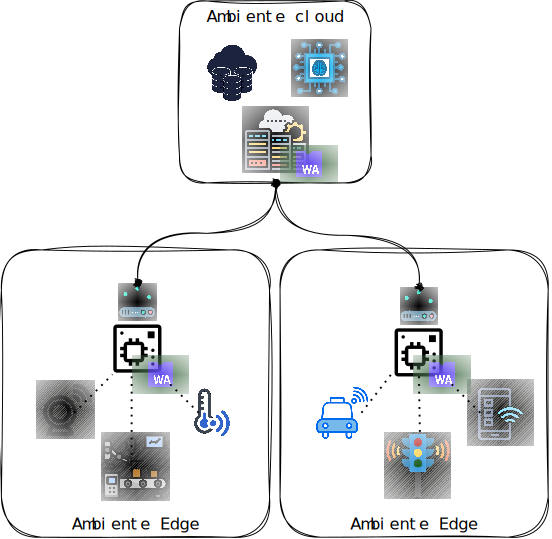
\includegraphics[width=0.8\textwidth]{img/schemi/schemi-Scenari.drawio.pdf}
    \caption{Modello Edge Computing}
    \label{fig:modello_edge_computing}
\end{figure}
\FloatBarrier

Per soddisfare i requisiti di migrazione e bilanciamento automatico fra nodi si è scelto di adottare wasmCloud, principalmente per i seguenti motivi:
\begin{itemize}
    \item Supporto all'esecuzione di componenti Wasm e specifica WASI Preview 2.
    \item Supporto sia di ambienti Cloud Native (come Kubernetes o Docker) che tradizionali (VM con Linux).
    \item Networking basato su rete mesh Lattice che consente di astrarre l'infrastruttura sottostante e permette l'interazione dei componenti.
    \item Cluster auto-rigenerante e facilmente scalabile all'interno del Lattice.
    \item Comunicazione efficiente grazie al backend basato su NATS.
    \item Gestione delle applicazioni tramite OCI Registry.
\end{itemize}

NATS è stata la soluzione selezionata anche per quanto riguarda la comunicazione e l'interazione delle applicazioni stesse, principalmente per il suo supporto alla clusterizzazione e alla distribuzione su ambienti edge basata su nodi Leaf.\\
L'infrastruttura completa può essere schematizzata come nella Figura \ref{fig:infra_wasmcloud_nats}.

\FloatBarrier
\begin{figure}[h]
    \centering
    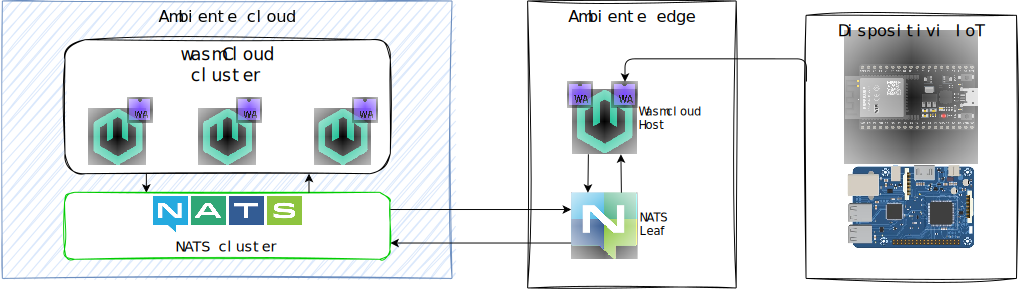
\includegraphics[width=\textwidth]{img/schemi/schemi-architettura-infra.drawio.pdf}
    \caption{Infrastruttura target}
    \label{fig:infra_wasmcloud_nats}
\end{figure}
\FloatBarrier

Il processo di trasformazione delle funzioni in componenti Wasm e la loro distribuzione verrà approfondita nella prossima sezione.

\section{PELATO Framework}

Lo scopo ultimo di questo elaborato è quindi trasformare una semplice funzione in un codice compilabile in componente Wasm, configurarlo in modo che possa essere deployato su ambienti wasmCloud e distribuirlo sull'infrastruttura.\\
La soluzione proposta è un framework denominato PELATO, acronimo di \textbf{Progettazione ed Esecuzione di Lifecycle Automatizzati e Tecnologie d'Orchestrazione per moduli WebAssembly}, che ha lo scopo di:

\begin{itemize}
    \item Fornire un modo intuitivo per istanziare un modulo FaaS, quindi ridurre al minimo le responsabilità dell'utilizzatore che dovrà esclusivamente specificare il codice della funzione da eseguire nella task remota.
    \item Consentire all'utilizzatore di configurare in modo intuitivo i metadati delle task, come il nome, il target di deployment, ma anche l'origine e la destinazione dei dati.
    \item Astrarre i più possibile il processo di generazione del codice e di Build del componente Wasm.
    \item Gestire il deployment dei componenti nell'infrastruttura.
\end{itemize}

Nelle seguenti sezioni verranno approfondite le scelte tecnologiche ed architetturali che sono state compiute durante la realizzazione di questo progetto.

\subsection{Tecnologie}

In questa sezione verranno elencate e spiegate le tecnologie utilizzate per lo sviluppo di questa soluzione. WebAssembly e gli argomenti correlati sono già stati ampiamente descritti nella sezione [\ref{sec:webassembly}], quindi ci concentreremo principalmente sui linguaggi e i tool utilizzati dal framework PELATO, come i linguaggi Python e Go.

\subsubsection{Python}

Il framework è stato implementato utilizzando Python, un linguaggio di programmazione ad alto livello interpretato ed orientato agli oggetti, apprezzato per la sua sintassi chiara e la tipizzazione dinamica che ne facilitano l'apprendimento e la manutenzione. Grazie a un vasto ecosistema di librerie è ampiamente utilizzato in ambiti come data science, sviluppo web e intelligenza artificiale. Supporta diversi paradigmi di programmazione e, grazie alla gestione automatica della memoria, riduce la complessità nello sviluppo. Inoltre, la sua portabilità su Windows, macOS e Linux lo rende adatto a molteplici contesti, dalla prototipazione rapida alle soluzioni enterprise.\\
È noto che Python, pur offrendo un ecosistema ricco e una sintassi intuitiva, può presentare limitazioni in termini di performance, soprattutto per operazioni CPU-intensive. Questo è in gran parte dovuto al Global Interpreter Lock (GIL), che impedisce l'effettivo sfruttamento del multi-threading in scenari di calcolo parallelo. Questi problemi sono stati risolti spostando il carico computazionale ed il parallelismo su strumenti esterni come Docker (la metodologia verrà spiegata in seguito).\\
La scelta di impiegare questo linguaggio per sviluppare il framework è stata motivata principalmente dalla vasta gamma di librerie disponibili. In particolare, per lo sviluppo di PELATO ce ne sono due fondamentali:
\begin{itemize}
    \item \textbf{Jinja}: è un motore di template per Python che permette di generare contenuti dinamici combinando testo statico e logica di programmazione. Utilizzato in framework web come Flask e strumenti di automazione come Ansible, trova applicazione anche nella configurazione di orchestratori come Helm, dove consente di parametrizzare file YAML. Attraverso la sintassi con doppie parentesi graffe, Jinja sostituisce variabili con valori definiti, rendendo la configurazione più flessibile e riutilizzabile. È stato utilizzato in fase di generazione del codice per parametrizzare lo stesso in base alla configurazione specificata dall'utente.
    \item \textbf{docker-py}: questa libreria consente di interagire con le API di Docker direttamente da Python, facilitando la gestione e l'automazione dei container. Permette operazioni come la creazione, l'avvio e l'eliminazione di container, oltre alla gestione di immagini e volumi. Questa integrazione è stata fondamentale per poter parallelizzare le operazioni di build e di deployment dei moduli Wasm.
\end{itemize}

\subsubsection{Golang}

Un altro linguaggio utilizzato è Go, noto anche come Golang, un progetto open source sviluppato da Google per offrire un equilibrio tra efficienza, sicurezza e semplicità. Grazie alla tipizzazione statica, al garbage collector e a un avanzato sistema di concorrenza basato sulle goroutine, Go consente la creazione di applicazioni scalabili e performanti. Pur supportando la programmazione orientata agli oggetti attraverso interfacce e struct, mantiene una sintassi essenziale e pragmatica. Inoltre, la sua ricca standard library fornisce strumenti per la gestione della rete, il parsing di file e la sicurezza crittografica.\\
Go è il linguaggio selezionato per la programmazione delle funzioni da eseguire nei componenti Wasm:
l'utente che utilizza il framework PELATO dovrà programmare i propri flussi utilizzando Go.\\
La scelta di utilizzare questo linguaggio è stata effettuata principalmente perché è uno dei due linguaggi (insieme a Rust) che attualmente implementa la specifica WASI Preview 0.2, necessaria per la composizione delle applicazioni tramite components e providers su wasmCloud.\\
La scelta di Go invece di Rust è avvenuta perché la sintassi di quest'ultimo risulta complessa e di difficile lettura, rendendolo meno accessibile per utenti senza esperienza pregressa. Al contrario, Go offre una sintassi più chiara e intuitiva, facilitando lo sviluppo e la manutenzione del codice.\\

\subsection{Struttura del framework}

In questa sezione verrà data una descrizione architetturale ad alto livello di PELATO. Il framework è sviluppato secondo un'architettura che adotta il pattern di progettazione \texttt{Facade} che fornisce un'interfaccia semplificata e unificata per accedere alle varie funzionalità. In pratica, una classe Facade funge da punto di accesso centrale, nascondendo la complessità interna e offrendo metodi di alto livello per interagire con il sistema.\\
La classe \texttt{Pelato} viene utilizzata come punto di accesso per la CLI (Command Line Interface), memorizza le configurazioni iniziali e si occupa di salvare le metriche. Inoltre è responsabile dell'esecuzione della logica di business implementata nei tre package:
\begin{itemize}
    \item \texttt{code\_generator}
    \item \texttt{wasm\_builder}
    \item \texttt{component\_deploy}
\end{itemize}

La configurazione iniziale della classe avviene tramite variabili d'ambiente (che possono essere caricate dal framework tramite un file \texttt{.env} locale, verranno dati più dettagli in seguito); ciò consente una facile implementazione del framework come applicazione containerizzata, nel caso si volesse ``trasformare" in un servizio gestito in Cloud.\\
Questo pattern di progettazione aumenta la modularità dei componenti facilitando eventuali estensioni, come quella mostrata nella Figura \ref{fig:pelato_architecture}, dove si fa l'esempio di un API Server affiancato alla CLI.\\

\FloatBarrier
\begin{figure}[h]
    \centering
    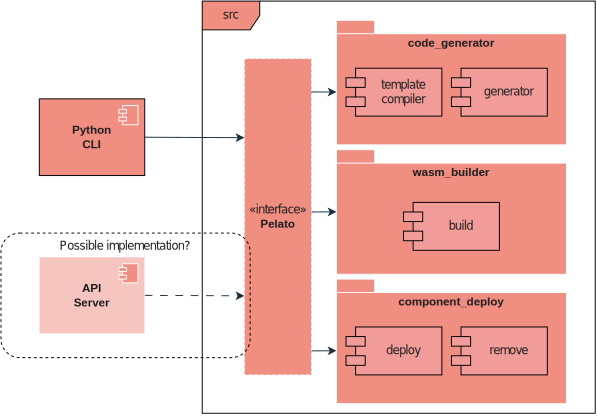
\includegraphics[width=0.8\textwidth]{img/schemi/schemi-implementazione-struttura.drawio.pdf}
    \caption{Architettura framework PELATO}
    \label{fig:pelato_architecture}
\end{figure}
\FloatBarrier

\section{Configurazione ed esecuzione framework}

In questa sezione verrà approfondita la configurazione del framework. Come già detto in precedenza il codice è scritto in Python, quindi sarà necessario avere un interprete di Python3 installato (consigliato \texttt{Python 3.12}), inoltre sarà necessario installare le librerie specificate nel \texttt{requirement.txt}. L'approccio consigliato è quello di utilizzare un virtual environment, cioè un'istanza dell'interprete Python che consente di installare le librerie localmente, senza toccare l'interprete configurato nel sistema o preoccuparsi di eventuali incompatibilità.\\
La configurazione dinamica avviene tramite variabili d'ambiente, ottenute dal sistema all'inizio di ogni esecuzione. Per facilitare il processo di configurazione è possibile creare un file \texttt{.env} situato nella cartella del framework: all'inizio di ogni esecuzione il file .env viene parsato e le variabili al suo interno vengono utilizzate per impostare il servizio.\\
All'interno della repository è predisposto il file \texttt{.env.template}, nel quale sono riportate le variabili d'ambienti impostabili e la configurazione di default, che viene mostrata nel Listing \ref{code:env}.

\begin{lstlisting}[language=bash, caption={Variabili d'ambiente per la configurazione del framework}, captionpos=b, label={code:env}]
    REGISTRY_URL=
    REGISTRY_USER=
    REGISTRY_PASSWORD=
    PARALLEL_BUILD=True
    NATS_HOST=localhost
    NATS_PORT=4222
    ENABLE_METRICS=True
\end{lstlisting}

Andiamo ad analizzarle:
\begin{itemize}
    \item \texttt{REGISTRY\_URL}, \texttt{REGISTRY\_USER}, \texttt{REGISTRY\_PASSWORD} servono per impostare le informazioni del registry in cui verranno caricate le immagini OCI dei moduli Wasm.
    \item \texttt{PARALLEL\_BUILD} abilita l'esecuzione dei container in modalità parallela.
    \item \texttt{NATS\_HOST} e \texttt{NATS\_PORT} sono utilizzati in fase di deployment e rappresentano l'istanza di NATS a cui il framework si collega per deployare le applicazioni sul cluster wasmCloud.
    \item \texttt{ENABLE\_METRICS} abilita la memorizzazione delle metriche ad ogni esecuzione del codice.
\end{itemize}

\subsection{Setup progetto}

L'utente finale, una volta configurato l'ambiente di esecuzione e impostate le variabili, per poter utilizzare il framework dovrà creare un progetto contenente:
\begin{itemize}
    \item Cartella \texttt{task} contenente i file Go in cui vengono definite le funzioni eseguite dai componenti Wasm.
    \item File \texttt{workflow.yaml} in cui inserire la configurazioni dei vari Task (per esempio nome, versione, template e nome del file Go) e sarà utilizzato dal generatore per compilare i template Jinja. Un esempio di file workflow viene mostrato nel Listing \ref{code:workflow_example}.    
\end{itemize}
Le modalità di compilazione di questi file verranno approfondite nel capitolo dedicato alla generazione del codice.

\begin{lstlisting}[language=yaml, caption={Esempio workflow.yaml}, captionpos=b, label={code:workflow_example}]
    project_name: Test_project
    tasks:
      - name: Temp sensor read
        type: producer_nats
        code: sensor_read.go
        targets:
          - cloud
          - edge
        source_topic: test_source_data
        dest_topic: test_dest_data
        component_name: temp_sensor_data
        version: 1.0.0
    ...
\end{lstlisting}

\subsection{PELATO CLI}

Come già anticipato in precedenza l'interfacciamento fra utente e framework è realizzata tramite una CLI, cioè un'interfaccia a riga di comando in grado di ricevere istruzioni e configurazioni.\\
Per invocare la CLI è sufficiente lanciare il comando \lstinline{python3 pelato.py}, che restituirà come output le varie opzioni e gli argomenti necessari, come mostrato nel Listing \ref{code:pelato_cli}.\\
\begin{lstlisting}[caption={Output Pelato CLI}, captionpos=b, label={code:pelato_cli}]
    usage: pelato.py [-h] {gen,build,deploy,remove,brush} ...
    Generate, build and deploy WASM components written in go
    
                        Command list
    gen                 Generate Go code
    build               Build WASM component
    deploy              Deploy WASM components
    remove              Remove deployed WASM components
    brush               Starts the pipeline: gen -> build -> deploy

    options:
      -h, --help            show this help message and exit
\end{lstlisting}

Ognuno di essi necessita come ulteriore argomento la path della cartella in cui sono contenuti il file \texttt{workflow.yaml} e le \texttt{task}. Nel Listing \ref{code:pelato_cli_examples} vengono riportati alcuni esempi di utilizzo.

\begin{lstlisting}[language=bash, caption={Cheatsheet comandi Pelato CLI}, captionpos=b, label={code:pelato_cli_examples}]
    $ python3 pelato.py -h      # help
    $ python3 pelato.py gen /home/lore/documents/project/   # generazione
    $ python3 pelato.py remove project/ # rimozione
    $ python3 pelato.py brush project/  # esecuzione pipeline
\end{lstlisting}

\section{Pipeline di esecuzione}

In questa sezione verrà descritta l'intera pipeline di esecuzione del framework, basandosi sui passaggi riportati nella Figura \ref{fig:pelato_pipeline}.

\FloatBarrier
\begin{figure}[h]
    \centering
    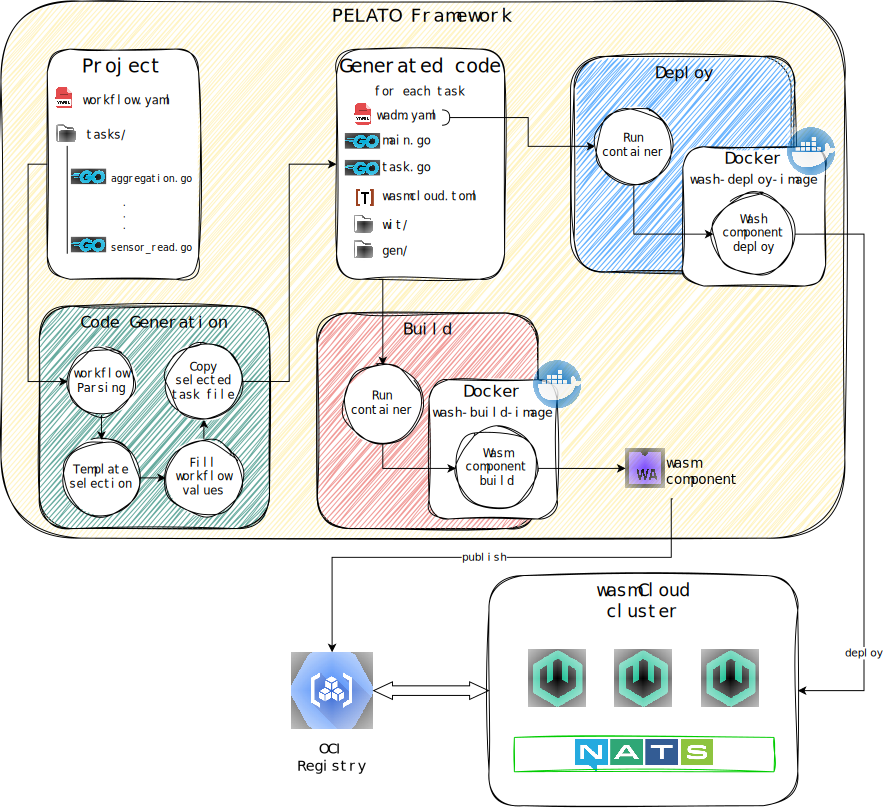
\includegraphics[width=0.9\textwidth]{img/schemi/schemi-arch-pipeline.drawio.pdf}
    \caption{Pipeline di esecuzione PELATO}
    \label{fig:pelato_pipeline}
\end{figure}
\FloatBarrier

Adesso verranno analizzati i tre componenti di esecuzione di PELATO:
\begin{enumerate}
    \item \textbf{Generazione}: in questa fase viene parsato il file \texttt{workflow.yaml} e poi utilizzato per generare i progetti Go necessari per buildare i moduli Wasm. Le configurazioni del file vengono utilizzate per selezionare il template di base, per sostituire i valori del template tramite Jinja e per identificare il file Go contenente la task. La struttura del progetto generato è mostrata nella Figura \ref{fig:pelato_pipeline} nell'area \texttt{Generated Code}.
    
    \item \textbf{Build}: questa fase si occupa di utilizzare i progetti Go generati in fase 1 e compilarli per ottenere un componente Wasm, quindi pubblicarlo come OCI artifact sul registry configurato. Queste operazioni avvengono all'interno di un container Docker nel quale sono installati tutti i tool necessari per l'operazione, come Go, TinyGo, Rust e wash.

    \item \textbf{Deploy}: è l'ultima fase della pipeline di PELATO, utilizza il manifest \texttt{wadm.yaml} generato in fase 1 per creare l'applicazione sulla piattaforma wasmCloud. Anche questa operazione avviene all'interno di un container in quanto necessita del tool wash.
\end{enumerate}

Una volta ultimato il processo, le applicazioni saranno disponibili sul wasmCloud, o lo diventeranno quando sarà presente un nodo healthy con label \texttt{host-type} corrispondente a quella selezionata dalla task.\\
La pipeline del framework è suddivisa nelle tre operazioni di generazione, build e deployment in modo che ognuna possa funzionare in modo autonomo (ovviamente se provviste delle risorse necessarie all'operazione). Inoltre, l'utilizzo di un container per le operazioni di build e deployment mira ad aumentare la compatibilità e la distribuzione del framework in modo che non sia dipendente dal sistema in cui verrà implementato: in questo progetto l'interfaccia è stata realizzata come CLI utilizzando Python, ma potrebbe essere anche esteso ad una configurazione SaaS completamente in Cloud o con approccio GitOps tramite actions e frameworks di CI/CD.\\
Tutte e tre le operazioni verranno approfondite nel dettaglio nei prossimi capitoli.

\chapter{Generazione}
In questo capitolo verrà approfondito il processo di generazione codice del progetto Go e del manifest wadm, che verranno impiegati poi per le fasi di Build e Deploy. Il primo passo è definire con precisione le struttura e la composizione dei file che fanno parte del progetto iniziale, quello che dovrà poi configurare l'utente finale che utilizzerà il framework, strutturato nel modo seguente:

\texttt{project/}
\dirtree{%
.1 workflow.yaml.
.1 tasks/.
.2 task1.go.
.1 gen/.
}

\section{Definizione Tasks}

In questa sezione ci si concentrerà sulle specifiche dei file task, cioè quelli situati nella cartella \texttt{tasks} del progetto e contenenti le funzioni che verranno eseguite dai moduli Wasm. Iniziamo fornendo la struttura base di ogni task file, mostrata nel Listing \ref{code:task_file}.
\begin{lstlisting}[language=Go, caption={Struttura base file task}, captionpos=b, label={code:task_file}]
    package main
    import (
    	...
    )
    ...    
    func exec_task(arg string) string{
    
    	return ... 
    }
\end{lstlisting}

I requisiti da rispettare per la definizione della task sono:
\begin{itemize}
    \item Il file deve avere un'estensione \texttt{.go}.
    \item Il package deve essere impostato su main (stesso package del main fornito dal template).
    \item Funzione di interfacciamento (cioè chiamata dal main) nominata \texttt{exec\_task}.
    \item La funzione di interfacciamento deve accettare una stringa e restituire una stringa.
\end{itemize}

La funzione interfaccia accetta e restituisce una stringa per facilitare il più possibile l'utilizzo da parte di un utente finale, che non dovrà preoccuparsi di tradurre i tipi Go con i tipi Wasm specificati in WASI (cosa che viene gestita in ``background'' sul file main del progetto Go).\\
Una volta soddisfatti questi requisiti è possibile eseguire innumerevoli operazioni, come importare librerie, definire strutture e altre funzioni. Un esempio è mostrato nel Listing \ref{code:task_file_json}, in cui viene importata la libreria \texttt{encoding/json} e definita una struct \texttt{Request}.

\begin{lstlisting}[language=Go, caption={Task file ed integrazione con Json}, captionpos=b, label={code:task_file_json}, keepspaces=true]
    package main
    import (
        "encoding/json"
    )
    type Request struct {
        Data int
        Name string
    }
    func exec_task(arg string) string{
        // unmarshal the data
        req := Request{}
        json.Unmarshal([]byte(arg), &req)
    
        // do some operations
        ...
        
        // return the json string
        json, _ := json.Marshal(req)
        return string(json)
    }
\end{lstlisting}

\section{Configurazione Workflow}

Passiamo ora alla codifica del file \texttt{workflow.yaml}, nel quale verranno effettivamente impostati i task e il loro comportamento. 

\subsection{Specifica file workflow}

Il file deve essere correttamente formattato in Yaml e contenere i seguenti campi:
\begin{itemize}
    \item \texttt{project\_name}: stringa contenente il nome del progetto, può contenere spazi e viene utilizzato principalmente nella CLI e nelle metriche.
    \item \texttt{tasks}: lista contenente i vari componenti Wasm.
\end{itemize}

Andando nel dettaglio, ogni elemento della lista \texttt{tasks} deve contenere:
\begin{itemize}
    \item \texttt{name}: stringa contenente il nome del componente, può contenere spazi e verrà impostato come nome dell'applicazione su wasmCloud.
    \item \texttt{type}: stringa contenente il template da utilizzare come base.
    \item \texttt{code}: stringa contenente il nome del file task da associare al componente Wasm in fase di generazione.
    \item \texttt{targets}: lista contenente delle stringhe che rappresentano la label \texttt{host-type} associata ai nodi target di deployment dei componenti Wasm.
    \item \texttt{source\_topic}: stringa contenente il topic da cui verranno ricevuti i dati.
    \item \texttt{dest\_topic}: stringa contenente il topic a cui verranno inviati.
    \item \texttt{component\_name}: stringa contenente il nome sintetico del componente, non può contenere spazi e funge da nome per l'OCI artifact associato.
    \item \texttt{version}: versione del componente, specificata nel formato \texttt{x.x.x}. Insieme al component\_name conferisce il nome all'OCI artifact.
    
\end{itemize}

\subsection{Template}

I template sono dei progetti già sviluppati che forniscono certe funzionalità e fungono da base per il codice fornito dall'utente. Attualmente sono implementati due template:
\begin{itemize}
    \item \texttt{processor\_nats}: comunicazione interamente basata su NATS: i dati arrivano da un topic e vengono inviati ad un topic.
    \item \texttt{http\_producer\_nats}: i dati possono provenire sia da un topic NATS che da una richiesta POST effettuata al nodo in cui è deployata l'applicazione. Viene utilizzato infatti l'http provider per esporre un web server nella porta 8000.
\end{itemize}

Questo approccio consente una facile estendibilità del progetto: infatti potranno essere sviluppati ed aggiunti nuovi template per aumentare le funzionalità disponibili sul framework. Un altro template attualmente in sviluppo è quello per la scrittura dei dati su un DB relazionale.\\
Per comprendere meglio le modalità di utilizzo del file workflow analizziamo un esempio.

\begin{lstlisting}[language=yaml, caption={Esempio Workflow file con processor e producer}, captionpos=b, label={code:workflow_file}, keepspaces=true]
project_name: Temperature data analysis
tasks:
  - name: Temp data conversion
    type: http_producer_nats
    code: convert.go
    targets:
      - edge
    source_topic: living_room_celsius_data
    dest_topic: living_room_kelvin_data
    component_name: celsius_to_kelvin_conversion
    version: 1.0.0
  - name: Data filter
    type: processor_nats
    code: filter.go
    targets:
      - cloud
    source_topic: living_room_kelvin_data
    dest_topic: filtered_kelvin_data
    component_name: temp_filter
    version: 1.0.2
\end{lstlisting}

Nel file workflow riportato nel Listing \ref{code:workflow_file} vengono definiti due componenti:
\begin{itemize}
    \item il primo si occupa di ricevere dati inviati da sensori ad un server http, convertire le temperature e pubblicarli in un topic NATS
    \item il secondo filtra i risultati, magari rimuovendo errori di misurazione o aggregandoli
\end{itemize}
Questo semplice esempio vuole mostrare come con una configurazione ridotta sia possibile generare, compilare e distribuire un'applicazione che supporta casi d'uso applicabili al mondo IoT.

\section{Generazione codice}

Il codice che si occupa della generazione è situato sul package \texttt{code\_generator} ed è distribuito nei file \texttt{generator.py} e \texttt{template\_compiler.py}. All'interno del package sono presenti anche i template utilizzati come base per i progetti Go, situati nella cartella \texttt{templates}.
\texttt{code\_generator/}
\dirtree{%
.1 .
.1 generator.py.
.1 template\_compiler.py.
.1 templates/.
.2 processor\_nats/.
.2 producer\_nats/.
}

\subsection{Parsing Workflow}

Verrà ora analizzato nel dettaglio il processo di generazione del codice, partendo dalla fase di analisi del progetto fornito dall'utente. La prima operazione viene effettuata da \texttt{generator.py}, di cui riportiamo un estratto contenente il codice più rilevante.
\begin{lstlisting}[language=python, caption={Generazione del codice}, captionpos=b, label={code:code_gen}]
    def generate(project_dir, registry_url, metrics, metrics_enabled):
        ...
        # Parsing del file workflow.yaml
        config = __parse_yaml(f"{project_dir}/workflow.yaml")
        
        # Pulizia della cartella di output
        __remove_dir_if_exists(output_dir)
        os.makedirs(output_dir, exist_ok=True)
        
        # Per ogni task all'interno del file workflow
        for task in config['tasks']:
            ...
            # Compilazione dei template
            template_compiler.handle_task(task, output_dir)

            # Copia del file task all'interno della cartella di output
            shutil.copy2(f"{project_dir}/tasks/{task['code']}", f"{output_dir}/{task['component_name']}/{task['code']}")
                
        if metrics_enabled:
            gen_metrics['gen_time'] = '%.3f'%(end_time - start_time)
            metrics['code_gen'] = gen_metrics
\end{lstlisting}

Come si può notare dal Listing \ref{code:code_gen} la funzione \texttt{generate} si occupa di parsare il file workflow, controllarne la validità e preparare la cartella di output. 

\subsection{Compilazione template}

La generazione vera e propria del codice viene affidata a \texttt{template\_compiler} tramite la funzione \texttt{handle\_task}, la quale seleziona il template corretto in base a quello riportato nella configurazione, lo copia nella cartella di output e lo compila utilizzando Jinja.\\
Nei Listing \ref{code:jinja_after} e \ref{code:jinja_after} viene riportato un esempio di file (in questo caso una porzione di \texttt{wadm.yaml}) prima e dopo la compilazione del template tramite Jinja.\\

\noindent\begin{minipage}{.46\textwidth}
\begin{lstlisting}[caption=Template wadm.yaml, language=yaml, basicstyle=\scriptsize, frame=single, label={code:jinja_before}]
spec:
  components:
    - name: {{ component_name }}
      type: component
      properties:
        image: "{{ registry_url }}/{{ component_name }}:{{ version }}"
      traits:
        - type: link
          properties:
            target: nats-processor
            namespace: wasmcloud
            package: messaging
            interfaces: [consumer]
        - type: spreadscaler
          properties:
            instances: 1
            spread:
            
            
            - name: {{ target }}
              weight: {{ weight }}
              requirements:
                host-type: {{ target }}
            
\end{lstlisting}
\end{minipage}
\hfill
$\rightarrow$
\hfill
\begin{minipage}{.46\textwidth}
\begin{lstlisting}[caption=wadm.yaml compilato con Jinja, language=yaml, basicstyle=\scriptsize, frame=single, label={code:jinja_after}]
spec:
  components:
    - name: data_double_test1
      type: component
      properties:
        image: "gitea.rebus.ninja/lore/data_double_test1:1.0.0"
      traits:
        - type: link
          properties:
            target: nats-processor
            namespace: wasmcloud
            package: messaging
            interfaces: [consumer]
        - type: spreadscaler
          properties:
            instances: 1
            spread:
            - name: cloud
              weight: 100
              requirements:
                host-type: cloud
\end{lstlisting}
\end{minipage}

A questo punto viene copiato il file specificato sulla configurazione dalla cartella \texttt{task/} del progetto alla cartella di output. La funzione viene automaticamente agganciata all'handler specifico del file main del template (dato che appartengono allo stesso package).\\

L'intero processo di generazione è stato schematizzato nella Figura \ref{fig:code_gen_impl}:

\FloatBarrier
\begin{figure}[h]
    \centering
    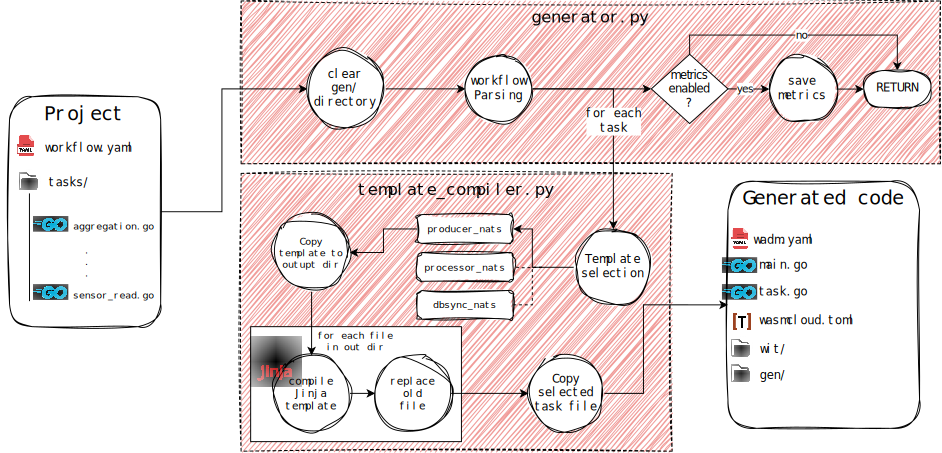
\includegraphics[width=\textwidth]{img/schemi/schemi-implementazione-gen.drawio.pdf}
    \caption{Processo generazione del codice}
    \label{fig:code_gen_impl}
\end{figure}
\FloatBarrier

\chapter{Build}
In questo capitolo verrà mostrato il processo che porta alla compilazione del processo Go in un componente Wasm.\\

Se la fase di generazione è avvenuta con successo, all'interno del progetto dovrebbe essere presente una cartella chiamata \texttt{gen}, contenente diverse sotto-cartelle con il codice necessario per compilare i moduli Wasm.

\texttt{project/}
\dirtree{%
.1 workflow.yaml.
.1 tasks/.
.1 gen/.
.2 example\_component1.
.2 example\_component2.
}

\section{Wasm Builder}

A questo punto può essere invocato il componente \texttt{build}, che sostanzialmente esegue le seguenti operazioni:
\begin{enumerate}
    \item Istanzia il client Docker utilizzando l'apposito SDK\footnote{\url{https://pypi.org/project/docker/}}.
    \item Controlla se l'immagine \texttt{wash-build-image:latest} è presente. Se non lo è procede a buildarla utilizzando il dockerfile configurato.
    \item Per ogni cartella presente dentro \texttt{gen} istanzia un container con \texttt{wash-build-image} come immagine e monta la cartella all'interno del container.
    \item Attende la terminazione dei container.
\end{enumerate}

Si può notare come in questo caso le operazioni svolte dal framework siano limitate: la logica di build del componente e la pubblicazione dell'artifact OCI sono infatti delegate alle istanze in esecuzione su Docker.
    
\subsection{Wash build image}

Approfondiamo ora il meccanismo utilizzato per compilare i componenti Wasm, iniziando dal Dockerfile che descrive l'immagine di base utilizzata, mostrato nel Listing \ref{code:wash_buil_image_dockerfile}.

\begin{lstlisting}[language=Dockerfile, caption={wash-build-image Dockerfile}, captionpos=b, label={code:wash_buil_image_dockerfile}, basicstyle=\ttfamily\small]
FROM ubuntu:24.04 AS wash-build-image

# Install dependencies and tools
RUN apt-get update && apt-get install -y curl wget tar ...

# ----------------- Install WasmCloud -----------------
RUN curl -s "https://packagecloud.io/install/repositories/wasmcloud/core/script.deb.sh" | bash && \
    apt-get install -y wash

# ----------------- Install Go 1.23 -----------------    
RUN wget https://go.dev/dl/go1.23.4.linux-amd64.tar.gz && \
    tar -C /usr/local -xzf go1.23.4.linux-amd64.tar.gz && \
    rm go1.23.4.linux-amd64.tar.gz

# Set Go environment variables
ENV PATH="/usr/local/go/bin:${PATH}"
ENV GOPATH="/go"
ENV GOROOT="/usr/local/go"

# ----------------- Install TinyGo 0.34.0 -----------------
RUN wget https://github.com/tinygo-org/tinygo/releases/download/v0.34.0/tinygo_0.34.0_amd64.deb && \
    dpkg -i tinygo_0.34.0_amd64.deb && \
    rm tinygo_0.34.0_amd64.deb

# ----------------- Install Rust -----------------
# Install Rust
RUN curl https://sh.rustup.rs -sSf | sh -s -- -y && \
    . "$HOME/.cargo/env" && \
    cargo install --locked wasm-tools

# Set Rust environment variables
ENV PATH="/root/.cargo/bin:${PATH}"

# Verify installations
RUN go version && tinygo version && cargo --version && wash --version && wasm-tools --version

# ----------------- Build the WasmCloud module -----------------
FROM wash-build-image

RUN mkdir /app
WORKDIR /app

# Install go dependencies, build the wasm module, push it to the registry
CMD ["sh", "-c", "go env -w GOFLAGS=-buildvcs=false && go mod download && go mod verify && wash build && wash push $REGISTRY build/*.wasm && chown -R ${HOST_UID}:${HOST_GID} ."]
\end{lstlisting}

Il Dockerfile è strutturato in due fasi:
\begin{enumerate}
    \item \textbf{Fase 1}: vengono installate le dipendenze di Go, TinyGo, Rust e la shell di wasmCloud.
    \item \textbf{Fase 2}: viene predisposta l'immagine per la compilazione dei moduli Wasm.
\end{enumerate}

La preparazione della compilazione avviene dentro l'istruzione CMD, che infatti contiene:
\begin{itemize}
    \item Istruzioni per risolvere le dipendenze di go ed installarle nel progetto. In questo modo l'utente può aggiungere librerie supportate e il builder si occuperà di installarle nel progetto.
    \item Comando \texttt{wash build} che esegue la compilazione del progetto e genera il componente Wasm all'interno della cartella \texttt{gen}.
    \item Comando \texttt{wash push} che pubblica il componente Wasm come artifact OCI sul registry passato come configurazione.
    \item Istruzione per impostare i permessi sui file generati, necessario per poter gestire correttamente i files tramite Python.
\end{itemize}

\subsection{Istanziamento container}

Questo approccio consente di utilizzare una sola immagine per tutte le operazioni di build: le configurazioni dinamiche avvengono tramite variabili d'ambiente e i file da buildare vengono montati come volume al posto della cartella \texttt{/app}, come possiamo notare dal Listing \ref{code:build} contenente un estratto di codice del componente \texttt{build}:

\begin{lstlisting}[language=python, caption={Build componente Wasm con Docker}, captionpos=b, label={code:build}]
def __build_wasm(task_dir, client, reg_user, reg_pass, detached, wait_list):
    oci_url = wadm['spec']['components'][0]['properties']['image']
    name = wadm['spec']['components'][0]['name'] + '-build'
    ...
    # Build componente Wasm
    print(f" - Building WASM module {oci_url}")
    container = client.containers.run(
        "wash-build-image:latest",
        environment=[f'REGISTRY={oci_url}',
                     f'WASH_REG_USER={reg_user}',
                     f'WASH_REG_PASSWORD={reg_pass}',
                     f'HOST_UID={uid}',
                     f'HOST_GID={gid}'],
        volumes={os.path.abspath(task_dir): {'bind': '/app', 'mode': 'rw'}},
        remove = True,
        detach = True,
        name = name
    )
    
    # Build sequenziale o parallela
    if detached == 'False':
        container.wait()
    else:
        wait_list.append(name)
\end{lstlisting}

\subsection{Esecuzione parallelizzata}

Il processo di build può essere eseguito in modalità sequenziale o parallela, a seconda della configurazione delle variabili d'ambiente. Questo comportamento è gestito tramite la flag \texttt{detach}, che permette di avviare i container in modo asincrono. In questa modalità, viene utilizzata una waiting list per istanziare tutti i container in parallelo e attendere il completamento dell'operazione di build.\\

\section{Processo completo}

L'intero processo di build viene mostrato nella Figura [\ref{fig:impl_build}]:

\FloatBarrier
\begin{figure}[h]
    \centering
    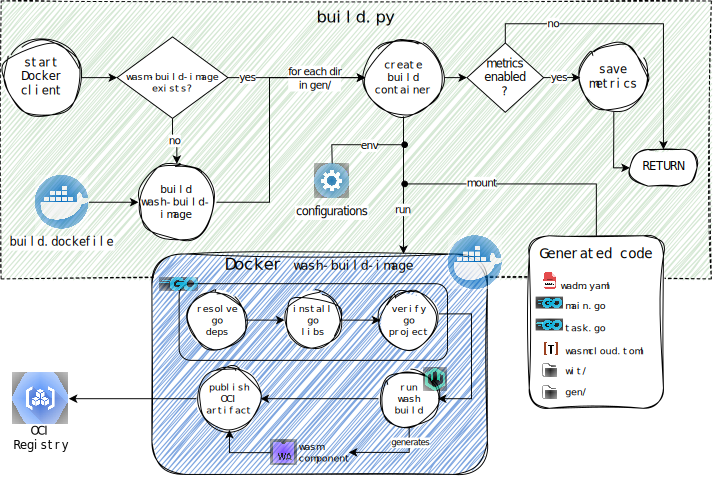
\includegraphics[width=\textwidth]{img/schemi/schemi-implementazione-build.drawio.pdf}
    \caption{Processo di Build componente Wasm}
    \label{fig:impl_build}
\end{figure}
\FloatBarrier

\chapter{Deployment}
In questo capitolo verrà descritta la procedura di deployment dei componenti Wasm nella piattaforma wasmCloud. La comunicazione fra questa ed il framework PELATO avviene tramite NATS: sarà sufficiente configurare il framework con le credenziali di un client NATS collegato al cluster per poter deployare le applicazioni.\\
Anche in questo caso il componente deploy si appoggia a Docker per l'operazione, dato che l'applicazione del deployment tramite il manifest \texttt{wadm.yaml} ottenuto in fase di Generazione deve essere effettuata utilizzando \texttt{wash}.

\section{Application Deployment}

La fase di deployment è strutturata in modo molto simile a quella di build, infatti le operazioni svolte dal componente deploy sono:

\begin{enumerate}
    \item Istanziamento del client Docker.
    \item Controllo dell'immagine \texttt{wash-deploy-image:latest}, se non è presente procede a buildarla utilizzando il dockerfile configurato.
    \item Per ogni cartella presente dentro \texttt{gen} istanzia un container con \texttt{wash-deploy-image} come immagine e monta la cartella all'interno del container.
    \item Attende la terminazione dei container.
\end{enumerate}

\subsubsection{Wash deploy image}

 Il Dockerfile utilizzato per buildare l'immagine \texttt{wash-deploy-image} è più semplice, in quanto deve solamente installare la wasmCloud shell e le sue dipendenze:
 
\begin{lstlisting}[language=Dockerfile, caption={wash-build-image Dockerfile}, captionpos=b, label={code:wash_buil_image_dockerfile}, basicstyle=\ttfamily\small]
FROM ubuntu:24.04 AS wash-deploy-image

# Install dependencies and tools
RUN apt-get update && apt-get install -y curl wget tar ...

# ----------------- Install WasmCloud -----------------
RUN curl -s "https://packagecloud.io/install/repositories/wasmcloud/core/script.deb.sh" | bash && \
    apt-get install -y wash

# ----------------- Deploy the WasmCloud module -----------------
FROM wash-deploy-image

RUN mkdir /app
WORKDIR /app

# Deploy the WasmCloud module
CMD ["sh", "-c", "wash app deploy wadm.yaml"]
\end{lstlisting}

\subsection{Deployer}

Il comando riportato nell'istruzione CMD in questo caso è \texttt{wash app deploy wadm.yaml}, che utilizza il file wadm.yaml per creare un'applicazione sul cluster wasmCloud specificato.\\
L'approccio utilizzato per eseguire i processi di deployment è analogo a quello della fase Build, la differenza sta nelle variabili d'ambiente necessarie all'operazione: in questo caso sarà necessario fornire hostname e porta di un server NATS collegato al cluster wasmCloud. Di seguito viene riportata la porzione di codice che si occupa di eseguire il container.\\

\begin{lstlisting}[language=python, caption={Deploy applicazione su wasmCloud}, captionpos=b, label={code:deploy}]
def __deploy_wadm(task_dir, client, nats_host, nats_port, detached, wait_list):
    path = os.path.abspath(task_dir) + '/wadm.yaml'
    name = wadm['spec']['components'][0]['name'] + '-deploy'
    ...
    # Deploy wasmCloud app
    print(f" - Deploying WASM module {name}")
    container = client.containers.run(
        "wash-deploy-image:latest",
        environment=[f'WASMCLOUD_CTL_HOST={nats_host}',
                     f'WASMCLOUD_CTL_PORT={nats_port}'],
        volumes={path: {'bind': '/app/wadm.yaml', 'mode': 'rw'}},
        remove=True,
        detach=True,
        name=name
    )
    
    if detached == 'False':
        container.wait()
    else:
        wait_list.append(name)
\end{lstlisting}

\subsection{Remover}

Nel package \texttt{component\_deploy} è presente anche la funzionalità \texttt{remove}, con codice e comportamenti analoghi a quella di deploy. L'unica differenza si presenta nel dockerfile, nel quale l'istruzione specificata nel CMD è \texttt{wash app remove wadm.yaml} e permette di rimuovere le applicazioni specificate sui file wadm dal cluster.\\

\section{Processo completo}

Anche in questo caso è possibile parallelizzare l'esecuzione dei container, sia in fase di deployment che di rimozione delle applicazioni. L'intero processo di deployment viene mostrato nella Figura \ref{fig:impl_build}.

\FloatBarrier
\begin{figure}[h]
    \centering
    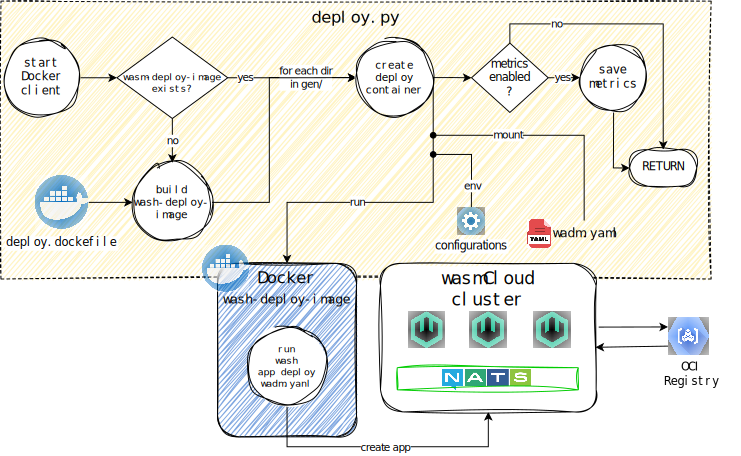
\includegraphics[width=\textwidth]{img/schemi/schemi-implementazione-deploy.drawio.pdf}
    \caption{Processo deployment applicazione su wasmCloud}
    \label{fig:impl_deploy}
\end{figure}
\FloatBarrier

\chapter{Valutazione performance}
In questo capitolo verrà utilizzato il framework sviluppato in questa tesi e ne verranno valutate le performance, andando ad analizzare il comportamento di ogni fase al variare del numero di task e con configurazioni diverse.

\section{Infrastruttura di test}

Iniziamo descrivendo l'infrastruttura in cui sono stati effettuati i test, specificando le modalità di deployment dei componenti architetturali come NATS e wasmCloud.

\subsection{Ambiente Cloud}

Per la simulazione di un ambiente Cloud è stato utilizzato un cluster Kubernetes composto da tre nodi, implementati su macchine virtuali con sistema operativo Ubuntu 22.04, eseguite all'interno dell'hypervisor Proxmox. La distribuzione adottata è K3s, con una configurazione in cui ciascun nodo assume simultaneamente il ruolo di Master e Worker, garantendo così un'architettura distribuita e resiliente.\\
Sia wasmCloud che il cluster NATS sono stati installati utilizzando un Helm Chart, cioè un pacchetto pre-configurato di risorse Kubernetes. Il Chart è fornito direttamente da wasmCloud\footnote{wasmCloud Platform: \url{https://github.com/wasmCloud/wasmCloud/tree/main/charts/wasmcloud-platform}} e consente di deployare:
\begin{itemize}
    \item \textbf{Cluster NATS} configurabile con più repliche.
    \item \textbf{NATS-Box}, Pod utilizzabile per accedere al cluster NATS ed effettuare dei test di performance.
    \item \textbf{wasmCloud Operator}, consente di deployare le applicazioni definite nei manifest \texttt{wadm} anche tramite CLI Kubernetes (\texttt{kubectl}) utilizzando delle CRD.
    \item \textbf{WADM} componente dell'ecosistema wasmCloud che si occupa di ricevere le richieste di wash e istanziare i moduli in base alle specifiche dei manifest \texttt{wadm}.
    \item \textbf{wasmCloud Host}, creato sulla base di una configurazione custom di Kubernetes\texttt{wasmCloudHostConfig} e punto di esecuzione dei componenti Wasm. Possono esserne create più repliche se necessario.
\end{itemize}
L'infrastruttura viene mostrata nella Figura \ref{fig:wasmcloud_platform}, ottenuta tramite il cluster manager Rancher collegato al cluster Kubernetes.

\FloatBarrier
\begin{figure}[h]
    \centering
    \includegraphics[width=\textwidth]{img/wasmcloud_platform_rancher.png}
    \caption{wasmCloud Platform su Kubernetes}
    \label{fig:wasmcloud_platform}
\end{figure}
\FloatBarrier


\subsection{Ambienti Edge}

Per simulare l'ambiente Edge sono stati utilizzati due semplici PC con sistema operativo Linux e provvisti di Docker Compose. L'host wasmCloud nei nodi Edge è stato deployato seguendo due modalità:
\begin{itemize}
    \item \textbf{Linux Service} istanziato tramite la wasmCloud Shell utilizzando il comando \lstinline{wash up -d --multi-local}.
    \item \textbf{Container} configurato tramite Docker Compose.
\end{itemize}

In entrambi i casi il collegamento con il cluster è stato effettuato utilizzando un nodo Leaf di NATS, deployato come container con la configurazione mostrata nel Listing \ref{code:nats_leaf_conf}.

\begin{lstlisting}[language=Python, caption={Configurazione nodo Leaf NATS}, captionpos=b, label={code:nats_leaf_conf}]
    jetstream {
      domain: leaf
    }
    leafnodes {
      remotes: [
        {
          url: "nats://nats.cluster.local:7422"     # Hostname del cluster NATS situato su Kubernetes
        }
      ]
    }
\end{lstlisting}

Per completare il flusso di esecuzione e simulare anche l'ambiente IoT sono stati utilizzati dei microcontrollori (come ESP32) collegati ai nodi Edge per produrre dati mock e metriche.\\
L'infrastruttura di test viene rappresentata nella Figura \ref{fig:infra_test} e può essere facilmente replicata grazie alle configurazioni presenti nella cartella \texttt{infra} del progetto.

\FloatBarrier
\begin{figure}[h]
    \centering
    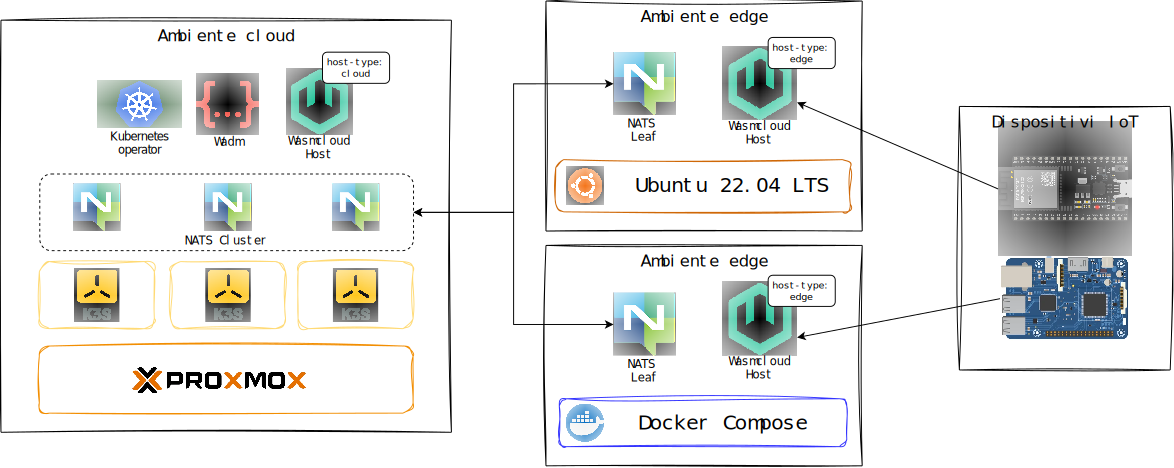
\includegraphics[width=\textwidth]{img/schemi/schemi-infrastuttura-impl.drawio.pdf}
    \caption{Infrastruttura di test}
    \label{fig:infra_test}
\end{figure}
\FloatBarrier

\subsection{Ambiente escuzione PELATO}

Il framework PELATO è stato eseguito all'interno di una delle macchine Edge. Per poter avere un'idea migliore delle performance del framework, riportiamo nel Listing \ref{code:hardware_spec} la configurazione hardware del PC in cui è stato eseguito.

\begin{lstlisting}[language=yaml, caption={Specifiche Hardware nodo Edge}, captionpos=b, label={code:hardware_spec}]
OS: Ubuntu 22.04 LTS x86_64 
Kernel: 6.11.0-17-generic
CPU: AMD Ryzen 7 7800X3D (8 cores 16 threads) 5.05 GHz
GPU: NVIDIA GeForce RTX 4070
Memory: 32 GiB DDR5 6000 MHz                                                        
\end{lstlisting}

Al momento della stesura di questo elaborato questa configurazione è considerabile high-end, quindi i grafici delle performance riportati nelle sezioni successive potrebbero essere ridimensionati in caso di esecuzione del framework in ambienti diversi, soprattutto nei casi di operazioni CPU-intensive come quella di build.

\section{Performance framework}

In questa sezione verranno mostrati i grafici e i risultati ottenuti sperimentando PELATO nell'infrastruttura descritta nella sezione precedente. Tutti i test che seguono sono stati misurati utilizzando la funzionalità di memorizzazione metriche integrata nel framework ed abilitabile con la variabile d'ambiente \texttt{ENABLE\_METRICS}. Inoltre, ogni test è stato eseguito almeno 5 volte e nei vari grafici viene riportato il confidence-interval al 95\% oltre al valore medio registrato.

\subsection{Startup Run}

Il primo test effettuato è stato quello di misurare la differenza nei tempi di esecuzione fra la prima volta e quelle successive: alla prima esecuzione del framework infatti dovrà anche buildare le immagini Docker utilizzate in fase di Build e Deploy.\\
Il test è stato effettuato lanciando PELATO su una configurazione di progetto minimale, con una singola task e codice con alcuna libreria aggiuntiva. Di seguito vengono riportati i grafici ottenuti analizzando le metriche della fase Build (Figura \ref{fig:test_startup_build}) e di quella Deploy (Figura \ref{fig:test_startup_deploy}). Sono state omesse le metriche della fase di Generazione in quanto non vi è alcuna differenza in quel caso fra la prima esecuzione e quelle successive.

\FloatBarrier
\begin{figure}[h]
    \centering
    \includegraphics[width=0.9\textwidth]{img/plots/barplot_startup_build.png}
    \caption{Tempo impiegato per la prima esecuzione di Build}
    \label{fig:test_startup_build}
\end{figure}
\FloatBarrier

Come è possibile vedere nella Figura \ref{fig:test_startup_build} i tempi di esecuzione cambiano drasticamente: il framework impiega circa 175 secondi aggiuntivi per buildare l'immagine \texttt{wash-build-image}, utilizzata nella fase di Build del componente Wasm. Questo comportamento è atteso, infatti l'immagine deve contenere tutti gli strumenti per compilare il progetto Wasm ed è necessario del tempo per poterli installare.

\FloatBarrier
\begin{figure}[h]
    \centering
    \includegraphics[width=0.9\textwidth]{img/plots/barplot_startup_deploy.png}
    \caption{Tempo impiegato per la prima esecuzione di Deploy}
    \label{fig:test_startup_deploy}
\end{figure}
\FloatBarrier

Un risultato più interessante è quello mostrato nella Figura \ref{fig:test_startup_deploy}: infatti il tempo di creazione dell'immagine \texttt{wash-deploy-image} è pressoché nullo. Questo è riconducibile alle ottimizzazioni effettuate dal Docker engine, infatti i layer dell'immagine precedentemente buildata \texttt{wash-build-image} rimangono in cache e vengono riutilizzati per costruire quella di deploy, che contiene esclusivamente il tool wash, riducendo drasticamente i tempi di esecuzione.

\subsection{Esecuzione parallela o sequenziale}

Il secondo test effettuato riguarda la differenza di performance fra le modalità di istanziamento dei container, cioè sequenziale o parallela. Le performance vengono misurate utilizzando il tempo di esecuzione per ogni fase.

\FloatBarrier
\begin{figure}[ht!]
    \centering
    \includegraphics[width=0.9\textwidth]{img/plots/gen_time_paired_barplot.png}
    \caption{Generazione codice sequenziale vs parallela}
    \label{fig:test_seq_par_gen}
\end{figure}
\FloatBarrier

\FloatBarrier
\begin{figure}[ht!]
    \centering
    \includegraphics[width=0.9\textwidth]{img/plots/build_time_paired_barplot.png}
    \caption{Build sequenziale vs parallela}
    \label{fig:test_seq_par_build}
\end{figure}
\FloatBarrier

\FloatBarrier
\begin{figure}[ht!]
    \centering
    \includegraphics[width=0.9\textwidth]{img/plots/deploy_time_paired_barplot.png}
    \caption{Deployment sequenziale vs parallela}
    \label{fig:test_seq_par_deploy}
\end{figure}
\FloatBarrier

\FloatBarrier
\begin{figure}[ht!]
    \centering
    \includegraphics[width=0.9\textwidth]{img/plots/total_time_paired_barplot.png}
    \caption{Pipeline PELATO sequenziale vs parallela}
    \label{fig:test_seq_par_total}
\end{figure}
\FloatBarrier

Analizziamo il comportamento del framework in base alle modalità:
\begin{itemize}
    \item Possiamo notare nella Figura \ref{fig:test_seq_par_gen} come la fase di Generazione non sia influenzata dalla modalità, comportamento atteso dato che non fa utilizzo dei container.
    \item La fase di Build è quella in cui è più evidente il vantaggio della parallelizzazione: sebbene la differenza sia poca per un numero di task basso, essa cresce esponenzialmente man mano che il numero sale, arrivando ad un tempo di esecuzione tre volte più basso rispetto alla modalità sequenziale, come mostrato nella Figura \ref{fig:test_seq_par_build}.
    \item Nella fase di Deploy si può notare un lieve miglioramento nella modalità parallelizzata, con una piccola discrepanza per n-task = 20 probabilmente dovuta ad un problema di connettività. Questo è osservabile nella Figura \ref{fig:test_seq_par_deploy}.
\end{itemize}

Osservando la Figura \ref{fig:test_seq_par_total}, che raffigura il tempo di esecuzione totale, possiamo osservare come la modalità parallelizzata sia in tutte le situazioni la scelta più efficiente e che sfrutta al meglio le risorse della macchina.

\subsection{Differenze fra template}

Durante la sperimentazione è emersa una leggera differenza nei tempi di esecuzione della pipeline in base al template scelto come base per i vari Task del file workload. Di seguito vengono riportati i grafici che paragonano i tempi di esecuzione del framework in base ai due template:
\begin{itemize}
    \item \texttt{processor\_nats}: utilizza esclusivamente il provider NATS.
    \item \texttt{http\_producer\_nats}: utilizza il provider NATS e anche il provider del web server HTTP.
\end{itemize}
Come si può vedere dalle figure \ref{fig:test_provider_gen}, \ref{fig:test_provider_build} e \ref{fig:test_provider_deploy}, i tempi di esecuzione sono leggermente più alti per il template con entrambi provider. Questo risultato è conforme alle aspettative, in quanto effettuare operazioni su più componenti risulta più oneroso per ogni parte della pipeline. Il risultato finale mostrato in Figura \ref{fig:test_provider_total} lo conferma.

\FloatBarrier
\begin{figure}[ht!]
    \centering
    \includegraphics[width=0.9\textwidth]{img/plots/gen_time_providers_barplot.png}
    \caption{Generazione codice, differenze fra template}
    \label{fig:test_provider_gen}
\end{figure}
\FloatBarrier

\FloatBarrier
\begin{figure}[ht!]
    \centering
    \includegraphics[width=0.9\textwidth]{img/plots/build_time_providers_barplot.png}
    \caption{Build, differenze fra template}
    \label{fig:test_provider_build}
\end{figure}
\FloatBarrier

\FloatBarrier
\begin{figure}[ht!]
    \centering
    \includegraphics[width=0.9\textwidth]{img/plots/deploy_time_providers_barplot.png}
    \caption{Deployment, differenze fra template}
    \label{fig:test_provider_deploy}
\end{figure}
\FloatBarrier

\FloatBarrier
\begin{figure}[ht!]
    \centering
    \includegraphics[width=0.9\textwidth]{img/plots/total_time_providers_barplot.png}
    \caption{Pipeline PELATO, differenze fra template}
    \label{fig:test_provider_total}
\end{figure}
\FloatBarrier

\subsection{Criticità}

In questa sezione verranno riportate le criticità riscontrate durante la fase di testing. Le prime discrepanze, come già accennato in una sezione precedente, appaiono durante l'analisi delle metriche della fase di Deploy. In alcuni casi i tempi di deployment delle applicazioni si scostano dalle previsioni (anche se di pochi secondi), probabilmente per problemi dovuti al sovraccarico della rete o del componente WADM del cluster wasmCloud.\\
Una criticità più importante è apparsa durante il test di esecuzione del framework in modalità parallelizzata con n-task \(\geq\) 15. Talvolta infatti l'esecuzione fallisce e la libreria di Docker restituisce la seguente eccezione
\begin{lstlisting}
     UnixHTTPConnectionPool(host='localhost', port=None): Read timed out. (read timeout=60)
\end{lstlisting}
probabilmente dovuta ad un sovraccarico della Unix Socket utilizzata da Docker. Per tamponare il problema è possibile aumentare il timeout della socket utilizzando le seguenti variabili d'ambiente
\begin{lstlisting}
DOCKER_CLIENT_TIMEOUT=120
COMPOSE_HTTP_TIMEOUT=120
\end{lstlisting}
e riavviando il servizio di Docker.

\section{Test Failover wasmCloud}

In questa sezione viene effettuato un test di recovery dopo il fallimento di un nodo. Lo scenario è composto da:
\begin{itemize}
    \item Cluster wasmCloud in un ambiente Cloud. Il wasmCloud Host è dotato di label \texttt{host-type: cloud}.
    \item Due ambienti Edge in reti separate, dotati di wasmCloud Host con label \texttt{host-type: edge}.
\end{itemize}

Il framework PELATO è stato usato per deployare un'applicazione che espone un web server HTTP (template http\_producer\_nats) utilizzando i file di configurazione mostrati nei Listing \ref{code:workflow_file_test} e \ref{code:task_file_test}, che descrivono un semplice use-case di un componente che riceve delle misurazioni della temperatura di una stanza tramite richieste HTTP, le converte da Celsius a Kelvin le pubblica su NATS. 

\begin{lstlisting}[language=yaml, caption={Workflow test recovery}, captionpos=b, label={code:workflow_file_test}, keepspaces=true]
project_name: Temperature data analysis
tasks:
  - name: Temp data conversion
    type: http_producer_nats
    code: convert.go
    targets:
      - edge
    source_topic: living_room_celsius_data
    dest_topic: living_room_kelvin_data
    component_name: celsius_to_kelvin_conversion
    version: 1.0.0
\end{lstlisting}

\begin{lstlisting}[language=Go, caption={Task file test recovery}, captionpos=b, label={code:task_file_test}, keepspaces=true]
    package main
    import (
    	"encoding/json"
    )
    type Request struct {
        Data float64
        Name string
    }
    func exec_task(arg string) string{
        req := Request{}
    	json.Unmarshal([]byte(arg), &req)
    	// Conversion between celsius and kelvin
    	req.Data = req.Data + 273.15
    	// return the json string
    	json, _ := json.Marshal(req)
    	return string(json)
    }
\end{lstlisting}

Il test effettuato vuole simulare la caduta di uno dei due nodi Edge (schematizzato in Figura \ref{fig:test_recovery}) e misurare il tempo impiegato dall'infrastruttura wasmCloud per accorgersi del problema e spostare l'esecuzione dell'applicazione sul nodo Edge funzionante.

\FloatBarrier
\begin{figure}[ht!]
    \centering
    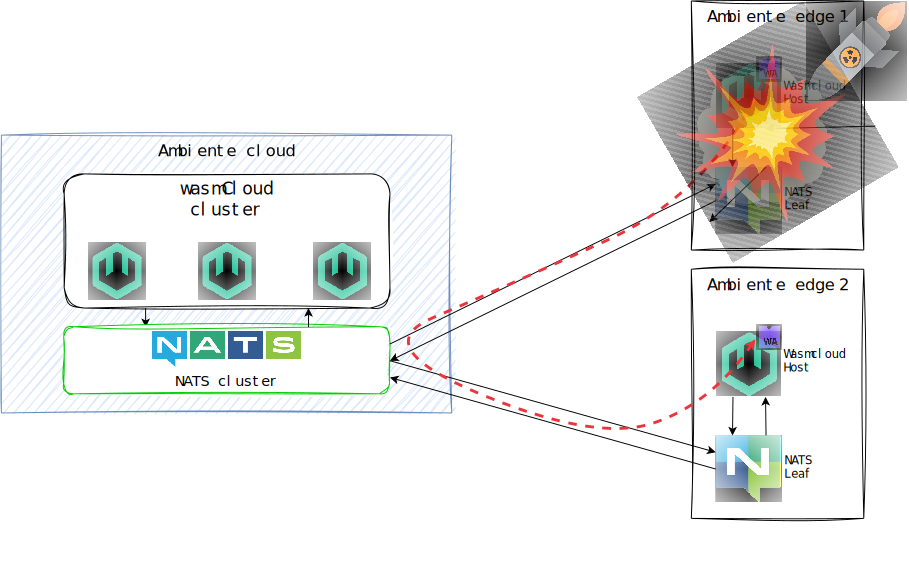
\includegraphics[width=0.75\textwidth]{img/schemi/schemi-test-failover-good.drawio.pdf}
    \caption{Scenario test failover}
    \label{fig:test_recovery}
\end{figure}
\FloatBarrier

I dati sono stati ottenuti misurando il tempo passato dalla distruzione del nodo 1 al deployment dell'applicazione sul nodo 2. L'applicazione viene considerata correttamente deployata quando il server HTTP risponde alla chiamata di test effettuata. Il nodo è stato cancellato stoppando il container in cui veniva eseguito il wasmCloud Host, la misurazione è stata effettuata tramite uno script bash che lancia comandi curl fino ad ottenere una risposta.\\
Dopo aver effettuato 5 test, il tempo di recovery si è assestato sui \(23 \pm 1.5\) secondi (come è possibile osservare dalla Figura \ref{fig:test_recovery_plot}), dimostrando come l'infrastruttura basata su wasmCloud possa rispondere alle perdite in tempi brevi.

\FloatBarrier
\begin{figure}[ht!]
    \centering
    \includegraphics[width=0.75\textwidth]{img/plots/boxplot_failover.png}
    \caption{Tempo di recovery wasmCloud}
    \label{fig:test_recovery_plot}
\end{figure}
\FloatBarrier

\chapter{Conclusioni}
Questo lavoro ha portato allo sviluppo di PELATO, un framework che rappresenta una soluzione innovativa per l’automazione e l’orchestrazione di moduli WebAssembly, adottando il paradigma Function as a Service (FaaS). PELATO consente di trasformare il codice in unità modulari ed eseguibili in maniera dinamica nell’Edge-Cloud Continuum, ottimizzando l’utilizzo delle risorse e migliorando la scalabilità in ambienti eterogenei. Attraverso l’adozione di tecnologie come Docker, Kubernetes e wasmCloud, PELATO combina l’efficienza dell’esecuzione quasi nativa dei moduli Wasm con la flessibilità necessaria per gestire carichi di lavoro complessi e dinamici.\\
Il framework è stato sviluppato seguendo un approccio strutturato che copre tre fasi principali: generazione, build e deployment. Nel capitolo dedicato alla generazione, viene affrontato il processo di configurazione e definizione dei workflow, con un focus sulla creazione automatizzata di task e sulla compilazione dei template Wasm. Questo consente agli sviluppatori di generare moduli Wasm in modo standardizzato e ottimizzato. Il capitolo dedicato alla build analizza il processo di compilazione dei moduli, implementando tecniche per ridurre i tempi di esecuzione, come la gestione delle immagini Docker in cache e l’esecuzione parallelizzata delle operazioni. Infine, il capitolo sul deployment esplora le strategie adottate per distribuire i moduli in ambienti Cloud ed Edge, sfruttando il modello a componenti di Wasm e il sistema di networking basato su NATS, che adotta il paradigma Pub/Sub per garantire comunicazioni affidabili e asincrone tra i componenti del sistema.\\
I risultati sperimentali evidenziano che PELATO è in grado di generare, buildare e deployare moduli Wasm garantendo prestazioni competitive in termini di tempi di avvio e overhead computazionale rispetto alle soluzioni containerizzate classiche. La validazione sperimentale è stata condotta attraverso quattro test principali, progettati per misurare le performance e la scalabilità del framework in diverse configurazioni operative, variando il numero di task, le modalità di esecuzione (sequenziale o parallelizzata) e la composizione delle applicazioni.\\
In modalità parallelizzata, PELATO ha mostrato tempi di esecuzione tre volte inferiori rispetto a quelli sequenziali, dimostrando una gestione ottimizzata per applicazioni con più task e una scalabilità lineare su piattaforme multi-core. Inoltre, la gestione delle immagini Docker in cache ha ridotto significativamente i tempi di avvio della fase di Build, migliorando l’efficienza complessiva del processo. Nei test di failover, il framework basato sull'infrastruttura wasmCloud ha evidenziato una capacità di recupero rapido, con un tempo medio di ripristino di 23±1,5 secondi dopo il fallimento di un nodo Edge. Questo approccio consente una gestione ottimizzata delle risorse, riducendo latenza e overhead, e garantisce una risposta tempestiva alle variazioni del carico di lavoro.\\
Integrandosi armoniosamente con infrastrutture moderne, PELATO facilita il deployment e la manutenzione delle applicazioni distribuite, eliminando la necessità di interventi manuali complessi. I tempi completi dell’esecuzione della pipeline con 20 task configurate si aggirano sui 175 secondi, un risultato in linea con i tempi di Build delle applicazioni containerizzate standard, confermando la competitività del framework rispetto alle soluzioni tradizionali.\\
Tra gli sviluppi futuri, si prevede l’implementazione di nuovi template che possano ampliare ulteriormente le funzionalità del framework. Questi template saranno progettati per semplificare la configurazione dei workflow e per favorire una più stretta integrazione con altri sistemi e tecnologie emergenti, come soluzioni di intelligenza artificiale, strumenti di monitoraggio avanzato e sistemi di persistenza dei dati. Tale evoluzione renderà il framework ancora più versatile e capace di adattarsi a una gamma più ampia di scenari applicativi, sfruttando appieno le potenzialità offerte dalla convergenza tra Cloud ed Edge.\\
Un ulteriore miglioramento potrebbe consistere nell’efficientamento delle procedure di build mediante l’adozione di container più minimali, in grado di ridurre ulteriormente l’overhead e migliorare i tempi di deploy dei moduli Wasm. Parallelamente, estendere il supporto a linguaggi diversi da Go rappresenta una prospettiva interessante: integrare toolchain per linguaggi come Rust, C++ e altri emergenti arricchirebbe la versatilità del framework, offrendo agli sviluppatori una gamma più ampia di opzioni per la generazione dei moduli e favorendo l’adozione della soluzione in contesti applicativi sempre più diversificati.\\
In conclusione, il framework PELATO rappresenta un contributo significativo all’orchestrazione dei moduli WebAssembly, offrendo una soluzione efficiente, resiliente e facilmente scalabile per la gestione delle applicazioni distribuite. I risultati ottenuti e le prospettive di sviluppo indicano un percorso di evoluzione continuo, che potrà ulteriormente potenziare l’efficacia della piattaforma e aprire nuove opportunità nel panorama del computing distribuito.

\listoffigures
\listoftables
\lstlistoflistings

\bibliographystyle{plain}
\bibliography{bibfile}

\myemptypage
\chapter*{Ringraziamenti}
\addcontentsline{toc}{chapter}{Ringraziamenti}

In primis, vorrei ringraziare il professore Marco Di Felice per l'opportunità che mi ha concesso, un ringraziamento particolare anche ad Ivan Zyrianoff per avermi seguito e supportato durante lo sviluppo e di questa tesi (probabilmente l'hai letta più volte di me).\\
Ringrazio i membri del Team 104 per la (poca) professionalità e i bei momenti passati insieme, non potevo chiedere un ambiente migliore per iniziare il mio percorso lavorativo.\\
Ringrazio anche l'Armata, i miei compagni di corso e tutti gli altri amici che mi sono stati vicino e che mi hanno fatto compagnia in questi cinque anni. Vi ringrazio per le uscite, i Gentoo party, le abbuffate di sushi e le lunghissime serate passate a nerdare.\\
Ringrazio i miei nonni, mio zio, i miei genitori e le mie sorelle: grazie per avermi supportato (e mantenuto) tutti questi anni, permettendomi di raggiungere questo traguardo. Grazie anche ai miei gatti grassi che mi hanno tenuto compagnia durante le ore di studio.\\ 
Ovviamente un ringraziamento speciale alla mia ragazza Chiara che, nonostante la distanza, è sempre riuscita a starmi accanto, spronandomi a studiare anche nei momenti di scarsa motivazione. Grazie anche per avermi aiutato a correggere la tesi (sicuramente l'hai letta più volte di me), senza il tuo supporto, non sarei mai arrivato fino a qui. :)

\end{document}